\documentclass[master=cws,masteroption=ai]{kulemt}
\setup{title={Algebraic Subtyping for Algebraic Types and Effects},
  author={Axel Faes},
  promotor={Prof.\,dr.\,ir.\ Tom Schrijvers},
  assessor={assesors},
  assistant={Amr Hany Saleh}}
% The following \setup may be removed entirely if no filing card is wanted
\setup{filingcard,
  translatedtitle=,
  udc=,
  shortabstract={}}

% Choose the main text font (e.g., Latin Modern)
\setup{font=lm}

%% Some recommended packages.
\usepackage{booktabs}   %% For formal tables:
                        %% http://ctan.org/pkg/booktabs
\usepackage{subcaption} %% For complex figures with subfigures/subcaptions
                        %% http://ctan.org/pkg/subcaption

\usepackage{array}
\usepackage{mathpartir}
\usepackage{xspace}
\usepackage{stmaryrd}
\usepackage{listings}
\usepackage{newtxmath}

%% Tikz Needed packages
\usepackage{pgfplots}
\pgfplotsset{width=7cm,compat=1.8}
\usepackage{pgfplotstable}
\renewcommand*{\familydefault}{\sfdefault}

% Finally the hyperref package is used for pdf files.
% This can be commented out for printed versions.
\usepackage[pdfusetitle,colorlinks,plainpages=false]{hyperref}

\input{tex/00-macros}
\newcommand{\todo}[1]{\textcolor{red}{\textsc{Todo:} #1}}

% Needed to use the files from spec
\let\subparagraph\paragraph
\let\paragraph\subsubsection
\let\subsubsection\subsection
\let\subsection\section
\let\section\chapter

\begin{document}

\begin{preface}
  I would like to thank everybody who kept me busy the last year,
  especially my promoter and my assistants. I would also like to thank the
  jury for reading the text.
\end{preface}

\tableofcontents*

\begin{abstract}
  Algebraic effects and handlers are a very active area of research. An important aspect is the development of an optimising compiler. \eff is an ML-style language with support for effects and forms the testbed for the optimising compiler. However, the type-\&-effect system of \eff is unsatisfactory. This is due to the lack of some elegant properties. It is also awkward to implement and use in practice.
\end{abstract}

\listoffigures
\listoftables

% Now comes the main text
\mainmatter

\section{Introduction}
Algebraic effects and handlers are a new formalism for formally modelling side-effects (e.g. mutable state or non-determinism) in programming languages, developed by Matija Pretnar (University of Ljubjana) and Gordon Plotkin (University of Edinburgh) \cite{DBLP:conf/lics/PlotkinP08,handling}. They can be seen as exception handlers on steroids. They look like exceptions and exception handlers. However, exception handlers have no way to access the continuation from where the exception was raised. Effect handlers do have this access. 

Algebraic effects and handlers are gaining a lot of traction, not only as a formalism but also as a practical feature in actual programming languages (e.g. the Koka language developed by Microsoft Research \cite{leijen2014koka}). We are collaborating with Matija Pretnar on the efficient implementation of one such language, called \eff. I have contributed to this collaboration during a project I did for the Honoursprogramme of the Faculty of Engineering Science.

Any typed programming language requires a type system in order to function. A type system governs a set of rules that assigns types to the various constructions in that typed programming language. Last year, in his December 2016 PhD thesis, Stephen Dolan (University of Cambridge, UK), has presented a novel type system that combines subtyping and parametric polymorphism in a particulary attractive and elegant fashion. A cornerstone of his design are the algebraic properties that the subtyping relation should respect. This system is called algebraic subtyping\cite{mlsub}

This thesis extends the algebraic subtyping approach in order to account for algebraic effects and handlers. The formal properties of this system are studied in order to find which properties are satisfied compared to other type-\&-effect systems. 

\section{Motivation}
Algebraic effects and handlers benefit from a custom type-\&-effect system, a type system that also tracks which effects can happen in a program. Several such type-\&-effect systems have been proposed in the literature \cite{leijen2014koka,handling,effectsystem}. We attribute this to the lack of the elegant properties of Dolan's type system. Indeed the existing type-\&-effect systems are not only theoretically unsatisfactory, but they are also awkward to implement and use in practice. This can be seen in recent research we did on an optimizing compiler for \eff \cite{optimization}. Within this research, the main hurdle here involved working with, instead of against, the type system of \eff based on subtyping. 

\paragraph{Research questions}
\begin{itemize}
\item How can Dolan's elegant type system be extended with effect information?
\item Which properties are preserved and which aren't preserved?
\item What advantages are there to an type-\&-effect system based on Dolan's elegant type system?
\end{itemize}

\section{Contributions}
The goal of this thesis, as well as it's main contribution, is to derive a type-\&-effect system that extends Dolan's elegant type system with effect information. This type-\&-effect system should inherit Dolan's harmonious combination of subtyping (in our case induced by a lattice structure on the effect information) with parametric polymorphism and preserve all of its desirable properties (both low-level algebraic properties and high-level meta-theoretical properties like type soundness and the existence of principal types). The following approach is taken:
\begin{enumerate}
\item Study of the relevant literature and theoretical background.
\item Design of a type-\&-effect system derived from Dolan's, that integrates effects.
\item Proving the desirable properties of the proposed type-\&-effect system: type soundness, principal typing, ...
\item Design of a type inference algorithm that derives the principal types of programs without type annotations and proving its correctness.
\item Implementation of the algorithm and comparing it to other algorithms.
\end{enumerate}

\section{Results}
A novel type-\&-effect system is provided. This system extends Dolan's algebraic subtyping system with effect information. The full specification for this system is given including terms, types, typing rules and equivalence rules to subtyping. A type inference algorithm for algebraic subtyping has also been extended to account for the effect information. This involves a type inference algorithm for the effects. Finally, another delivarable is an implementation of this system within the \eff programming language. This is a fully featured programming language that is and can be used for further evaluation and comparisons.

\section{Structure of the thesis}
\textbf{Chapter~\ref{background}} provides the required background in programming language theory, algebraic effects and optimizing \eff. How a type system specification needs to be read can be found in the section about programming language theory. This section explains the simply typed lambda calculus which is the simplest typed calculus. This calculus is the foundation for the calculus given in the section about algebraic effects. 

The section about algebraic effects gives the calculus of \eff and an thorough explanation of algebraic effects and handlers. The final section explains the research that led to this thesis, the optimization of \eff. An explanation of the optimization techniques are given and the hurdles encountered during the research are explained. 

\textbf{Chapter~\ref{core},~\ref{type-inference} and~\ref{simplification}} define the \core type system. This is the main constribution of this thesis. The major novelty is the representation and construction of the effect information. \textbf{Chapter~\ref{core}} gives the concrete syntax and the typing rules of the \core type system. 

\textbf{Chapter~\ref{type-inference}} introduces polar types and presents the algorithm to infer principal types and the biunification algorithm. Biunification is an analogue of unification for solving subtyping constraints. The difference is that biunification works over polar types. 

\textbf{Chapter~\ref{simplification}} shows how types and effects may be represented compactly as automata. This representation is an extension from the representation from Algebraic Subtyping. The automata is used in order to simplify types in order to give smaller types.

\textbf{Chapter~\ref{implementation}} explains the empirical work that is done. This includes an explanation of the \eff programming language and gives implementation details of the \core type system. Finally, the evaluation of the \core system is given as the system is compared with subtyping.

\textbf{Chapter~\ref{related}} reviews related work such as explicit eff subtyping, and \textbf{Chapter~\ref{conclusion}} presents some future work and concludes the thesis. Proofs are given in \textbf{Appendix~\ref{proofs}}.

\section{Background}
\subsection{Programming language theory}
The field of programming language theory is a branch of computer science that describes how to formaly define complete programming languages and programming language features, such as algebraic effect handlers.

The work described in this thesis uses several aspects from programming language theory. An important subdiscipline that is extensively used is type theory. Type theory is used to formaly describe type systems. A type system is a set of rules that are used to define the shape of meaningful programs. The \textit{simply typed lambda calculus} will be used to show and explain the necessary background that is required for further chapters. The \textit{simply typed lambda calculus} is the simplest and most elementary form of all typed languages. \cite{pierce2002types}

\subsection{Types and terms}

\paragraph{Terms}
Figure~\ref{fig:terms:lambda} shows the three sorts of terms of the \textit{simply typed lambda calculus}. A variable by itself is already a term. The abstraction of some variable $x$ from a certain term $t$ is called a function. Finally, an application is a term. The terms define the syntax of a programming language, but it does not place any constraints on how these terms can be composed. A wanted constraint could for example be that an application $t_1 \, t_2$ should only be valid if $t_1$ is a function. This shows that only having terms is not enough to describe a programming language. \cite{hindley1986introduction}

\begin{figure}[!htb]
\begin{center}
\framebox{
\begin{minipage}{0.98\columnwidth}
\[\begin{array}{r@{~}c@{~}l@{\quad}l}
  \text{terms}~t & \bnfis {} & x & \text{variable} \\
    & \bnfor & \tru & \text{true} \\
    & \bnfor & \fls & \text{false} \\
    & \bnfor & \fun{x \T T} t & \text{function} \\
    & \bnfor & t_1 \, t_2 & \text{application}
\end{array}\]
\end{minipage}
}
\end{center}
\caption{Terms of simply typed lambda calculus}\label{fig:terms:lambda}
\end{figure}

\paragraph{Types}
Since the \textit{simply typed lambda calculus} is being used, types are needed. As seen in figure~\ref{fig:types:lambda}, there are two types, the base type and the function type. In a valid and meaningful program, every term has a type. A term is called well typed or typable if there is a type for that term. 

\begin{figure}[!htb]
\begin{center}
\framebox{
\begin{minipage}{0.98\columnwidth}
\[\begin{array}{r@{~}c@{~}l@{\quad}l}
  \text{type}~T & \bnfis {}
    & bool & \text{base type} \\
    & \bnfor & T \to T & \text{function type}
\end{array}\]
\end{minipage}
}
\end{center}
\caption{Types of simply typed lambda calculus}\label{fig:types:lambda}
\end{figure}

\subsection{Typing rules}

As stated above, a method is needed to place constraints on the programming language. This is done with typing rules or types judgements. The typing rules for the \textit{simply typed lambda calculus} are given in figure~\ref{fig:lambda-typing}. 

\begin{figure}[!htb]
\begin{center}
\framebox{
\begin{minipage}{0.95\columnwidth}
\[\begin{array}{r@{~}c@{~}l}
  \text{typing contexts}~\ctx & \bnfis {} & \epsilon \bnfor \ctx, x : T \\
\end{array}\]
\begin{mathpar}
  \inferrule[True]{
  }{
    \ctx \ent \tru \T bool
  }

  \inferrule[False]{
  }{
    \ctx \ent \fls \T bool
  }

  \inferrule[Var]{
    (x \T T) \in \ctx
  }{
    \ctx \ent x \T T
  }

  \inferrule[App]{
    \ctx \ent t_1 \T T_1 \to T_2 \\
    \ctx \ent t_2 \T T_1
  }{
    \ctx \ent t_1 \, t_2 \T T_2
  }
  
  \inferrule[Fun]{
    \ctx, x \T T_1 \ent t \T T_2
  }{
    \ctx \ent \fun{x \T T} t \T T_1 \to T_2
  }
\end{mathpar}
\end{minipage}
}
\end{center}
\caption{Typing of simply typed lambda calculus}\label{fig:lambda-typing}
\end{figure}

The first rules to take note of are the \textsc{True} and \textsc{False} rules. These are facts and state that the terms true and false have type \textit{bool}. A \textit{Fact} states that, under the assumption of $\ctx$, $t$ has type $T$. The context, $\ctx$, is a mapping of the free variables of $t$ to their types. It is called a fact since the rule always holds.

The context, $\ctx$, is a (possibly empty) collection of variables mapped to their types. The \textsc{Var} rule states that, if the context contains a mapping for a variable, that variable is also a valid term with that type. The \textsc{App} rule defines the usage of a function. When there are two terms $t_1$ and $t_2$ with types $T_1 \to T_2$ and $T_1$, then the application $t_1 \, t_2$ will have the type $T_2$.  

An inference rule can be read in multiple ways. It can be read top-down or bottom-up. Reading it top-down gives the above described reasoning. Given some expressions and some constraints, another expression can be constructed with a specific type. The bottom-up approach states that, given an expression such as the function application, there is a specific way the different parts of the expression can be typed. In the \textsc{App} rule, a function expression has type $T_2$. Therefor, both $t_1$ and $t_2$ must follow a specific set of constraints. It is known that a function needs to exist of type $T_1 \to T_2$ and an expression that matches the argument of the function, $T_1$ needs to exist. \cite{pierce2002types}

Finally, there is the \textsc{Fun} rule. This rule is also called a function abstraction or simply an abstraction. It shows how a function can be constructed. The interesting part of this rule is $\ctx, x \T T_1 \ent t \T T_2$. This states that $t$ is only entailed by some context and a variable of type $T_1$.

\subsection{Other extensions}

Now, a full specification of the \textit{simply typed lambda calculus} is given. However, there are many extensions that can be added onto this language. In the next chapter, \eff will be discussed. \eff is a language which can be described as a modification of the \textit{simply typed lambda calculus} with algebraic effects and handlers. \eff is also uses subtyping rules, this concept will also be further explained in the next chapter. After this, algebraic subtyping will be added to the language.

Of course, just a specification does not have much meaning. Certain aspects or properties could be proved in order to show that they do (or do not) hold in the given language. Type inference is another aspect which is not talked about in this chapter. Type inference revolves around the automatic detection (or inference) of the types of terms. Both proofs and a type inference algorithm are given in later chapters. 

\section{Related Work (Algebraic Subtyping)}
Subtyping is a partial order which is a reflexive transitive binary relation satisfying antisymmetry (subtyping rules). The subtyping order also forms a distributive lattice (equivalence rules). 



\section{Related Work (\eff)}
Algebraic effect handling is a very active area of research. Implementations of algebraic effect handlers are becoming available and the theory is actively being developed. The type-\&-effect system that is used in \eff is based on subtyping and algebraic effect handlers \cite{effectsystem}. The \textit{simply typed lambda calculus} is used as a basis for \eff.  Let us start with a simple example in order to show what algebraic effects and handlers are. With this example, the differences with the \textit{simply typed lambda calculus} can also be shown.

In the example below, a new effect is defined \textit{DivisionByZero}. In essence, this effect can be thought of as an exception. From the type that is written, it can also be seen that an exception has some relation with functions. In this case, the effect describes a function type from \textit{unit} to \textit{empty}. This type describes what kind of argument the effect requires in order to be called and what kind of type it leaves behind after being handled. 

\begin{lstlisting}[language=Caml]
effect DivisionByZero : unit -> empty;;

let divide a b = 
  if (b == 0) then 
    #DivisionByZero () 
  else 
    a / b;;

let safeDivide a b = 
  handle (divide a b) with 
    | #DivisionByZero () k -> 0;;
\end{lstlisting}

The effect can be called just like any function can be called, by applying an argument to it. Here, an important distinction can be made. Any term that can contain effects are called computations and are dirty, while terms that cannot contain effects are called expressions and are pure. Finally, computations can be handled. This can be thought of as an exception handler with the big difference being that within an effect handler, there is access to a continuation to the place where the effect was called. 

To reiterate, in order to extend \textit{simply typed lambda calculus} to \eff, several terms need to be added. A term is required in order to call effects and handle effects. Of course, we need to be able to have handlers as well. \cite{pretnar2015introduction}




\subsection{Types and terms}

\paragraph{Terms}
Figure~\ref{fig:terms:eff} shows the two kinds of terms in \eff. As explained before, there are values $v$ and computations $c$. Computations are terms that can contain effects. Effects are denoted as operations $Op$ which can be called. \cite{handling}

In \eff, there are also several other small additions aside from the terms required for the algebraic effects and handlers. Sequencing, a conditional and a recursive definition have also been added. This was done in order to enrich the language and further exploit the advantage of algebraic effects and handlers. \cite{programming}

\begin{figure}[!htb]
\begin{center}
\framebox{
\begin{minipage}{0.98\columnwidth}
\[\begin{array}{r@{~}c@{~}l@{\quad}l}
  \text{value}~v & \bnfis {} & x & \text{variable} \\ %\lambda\text{-variable} \\
    % & \bnfor & \letvar & \text{let-variable} \\
    % & \bnfor & \const & \text{constant} \\
    & \bnfor & \tru & \text{true} \\
    & \bnfor & \fls & \text{false} \\
    & \bnfor & \fun{x} c & \text{function} \\
    & \bnfor & \{ & \text{handler} \\
    & & \quad \ret x \mapsto c_r, & \quad\text{return case} \\
    & & \quad \shortcases & \quad\text{operation cases} \\
    & & \} & \\ 
  \text{comp}~c & \bnfis & v_1 \, v_2 & \text{application} \\
    & \bnfor & \doin{x \leftarrow c_1} c_2 & \text{sequencing} \\
    & \bnfor & \conditional{e}{c_1}{c_2} & \text{conditional} \\
    & \bnfor & \letrecin{f \, x = c_1} c_2 & \text{rec definition} \\
    & \bnfor & \ret v  & \text{returned val} \\
    & \bnfor & \op \, v & \text{operation call} \\
    & \bnfor & \withhandle{v}{c} & \text{handling}
\end{array}\]
\end{minipage}
}
\end{center}
\caption{Terms of \eff}\label{fig:terms:eff}
\end{figure}

\paragraph{Types}
Figure~\ref{fig:types:eff} shows the types of \eff. There are two main sorts of types. There are (pure) types $A, B$ and dirty types $\C, \D$. A dirty type is a pure type $A$ tagged with a finite set of operations $\dirt$, which we call dirt, that can be called. This finite set $\dirt$ is an over-approximation of the operations that are actually called. The type $\C \hto \D$ is used for handlers because a handler takes an input computation $\C$, handles the effects in this computation and outputs computation $\D$ as the result \cite{handling}. Other than the handler type and the distinction between pure and dirty types, there is nothing new compared to the types from the \textit{simply typed lambda calculus}.

\begin{figure}[!htb]
\begin{center}
\framebox{
\begin{minipage}{0.98\columnwidth}
\[\begin{array}{r@{~}c@{~}l@{\quad}l}
  \text{(pure) type}~A, B & \bnfis {}
    % & \boolty \bnfor \intty & \text{basic types} \\
    & \boolty & \text{bool type} \\
    & \bnfor & A \to \C & \text{function type} \\
    & \bnfor & \C \hto \D & \text{handler type} \\
  \text{dirty type}~\C, \D & \bnfis {} & A \E \dirt \\
  \text{dirt}~\dirt & \bnfis {} &\set{\op_1, \dots, \op_n}
\end{array}\]
\end{minipage}
}
\end{center}
\caption{Types of \eff}\label{fig:types:eff}
\end{figure}

\subsection{Subtyping}
\eff uses a subtyping based system. Subtyping is a form of type polymorphism. Types can be related to eachother, being either subtypes or supertypes. Intuitively one could think about Java classes and inheritance in order to understand subtyping. There are some big differences between inheritance and subtyping, but from the principle of gaining an understanding of what subtyping entails, the relation between the two can be made. 

Let us take the subtyping judgement $\boolty \le \boolty$. This judgement is about reflexivity. It states that $\boolty$ is a subtype of itself. The subtyping judgement for the arrow type (functions) states that, if we have $A' \le A$ and $\C \le \C'$, then we also induce the natural subtyping judgement $A \to \C \le A' \to \C'$. This tells us that, if we have a function, the caller can always call that function with a type that is "more" and that function can always return "more" than what the caller expects. This can be easily visualised when the argument and return values are records. If a function requires a record with labels "x" and "y", the caller is allowed to call the function with a record containing more that just "x" and "y". A similar analogy can be made for the return values. Functions are contravariant in its argument types and covariant in its return types.

The dirty type $A \E \dirt$ is assigned to a computation returning values of type $A$ and potentially calling operations from the set $\dirt$. This set $\dirt$ is always an over-approximation of the actually called operations, and may safely be increased, inducing a natural subtyping judgement $A \E \dirt \le A \E \dirt'$ on dirty types where $\dirt'$ contains extra operations compared to $\dirt$. As dirty types can occur inside pure types, we also get a derived subtyping judgement on pure types. Both judgements are defined in Figure~\ref{fig:subtyping}. Observe that, as usual, subtyping is contravariant in the argument types of functions as well as handlers, and covariant in their return types. \cite{inferring}

\begin{figure}[!htb]
\begin{center}
\framebox{
\begin{minipage}{0.95\columnwidth}
\textbf{Subtyping}
\begin{mathpar}
  \inferrule[Sub-$\boolty$]{
  }{
    \boolty \le \boolty
  }

  \inferrule[Sub-$\to$]{
    A' \le A \\
    \C \le \C'
  }{
    A \to \C \le A' \to \C'
  }

  \inferrule[Sub-$\hto$]{
    \C' \le \C \\
    \D \le \D'
  }{
    \C \hto \D \le \C' \hto \D'
  }

  \inferrule[Sub-$\E$]{
    A \le A' \\
    \dirt \subseteq \dirt'
  }{
    A \E \dirt \le A' \E \dirt'
  }
\end{mathpar}
\end{minipage}
}
\end{center}
\caption{Subtyping for pure and dirty types of \eff}\label{fig:subtyping}
\end{figure}

\subsection{Typing rules}
Figure~\ref{fig:eff-typing:e} and figure~\ref{fig:eff-typing:c} defines the typing judgements for values and computations with respect to a standard typing context $\ctx$. This types context can contain $\epsilon$ or a variable with a type.

\paragraph{Values}
The rules for subtyping, variables, and functions are entirely standard.

A handler expression has type $A \E \dirt \cup \ops \hto B \E \dirt$ iff all branches (both the operation cases and the return case) have dirty type $B \E \dirt$ and the operation cases cover the set of operations $\ops$. Note that the intersection $\dirt \cap \ops$ is not necessarily empty. The handler deals with the operations $\ops$, but in the process may re-issue some of them (i.e., $\dirt \cap \ops$).

When typing operation cases, the given signature for the operation $(\op \T A_\op \to B_\op) \in \sig$ determines the type $A_\op$ of the parameter $x$ and the domain $B_\op$ of the continuation $k$. As our handlers are deep, the codomain of $k$ should be the same as the type $B \E \dirt$ of the cases. \cite{inferring}

\paragraph{Computations}
With the following exceptions, the typing judgement $\ctx \ent c : \C$ has a straightforward definition. The $\ret$ construct renders a value $v$ as a pure computation, i.e., with empty dirt. An operation invocation $\op\,v$ is typed according to the operation's signature, with the operation itself as its only operation. Finally, rule \textsc{With} shows that a handler with type $\C \hto \D$ transforms a computation with type $\C$ into a computation with type $\D$. \cite{inferring}

\begin{figure}[H]
\begin{center}
\framebox{
\begin{minipage}{0.95\columnwidth}
\[\begin{array}{r@{~}c@{~}l}
  \text{typing contexts}~\ctx & \bnfis {} & \epsilon \bnfor \ctx, x : A\\
\end{array}\]
\textbf{Expressions}
\begin{mathpar}
  \inferrule[SubVal]{
    \ctx \ent v \T A \\
    A \le A'
  }{
    \ctx \ent v \T A'
  }

  \inferrule[Var]{
    (x \T A) \in \ctx
  }{
    \ctx \ent x \T A
  }

  % \inferrule[Const]{
  %   (\const \T A) \in \sig
  % }{
  %   \ctx \ent \const \T A
  % }

  \inferrule[True]{
  }{
    \ctx \ent \tru \T bool
  }

  \inferrule[False]{
  }{
    \ctx \ent \fls \T bool
  }
  
  \inferrule[Fun]{
    \ctx, x \T A \ent c \T \C
  }{
    \ctx \ent \fun{x} c \T A \to \C
  }

  \inferrule[Hand]{
    \ctx, x \T A \ent c_r \T B \E \dirt \\
    \Big[
      (\op \T A_\op \to B_\op) \in \sig \qquad \\
      \ctx, y \T A_\op, k \T B_\op \to B \E \dirt \ent c_\op \T B \E \dirt
    \Big]_{\op \in \ops}
  }{
    \ctx \ent \shorthand \T \\ A \E \dirt \cup \ops \hto B \E \dirt
  }
\end{mathpar}
\end{minipage}
}
\end{center}
\caption{Typing of expressions in \eff}\label{fig:eff-typing:e}
\end{figure}

\begin{figure}[H]
  \begin{center}
  \framebox{
  \begin{minipage}{0.95\columnwidth}
  \[\begin{array}{r@{~}c@{~}l}
    \text{typing contexts}~\ctx & \bnfis {} & \epsilon \bnfor \ctx, x : A\\
  \end{array}\]
\textbf{Computations}
\begin{mathpar}
  \inferrule[SubComp]{
    \ctx \ent c \T \C \\
    \C \le \C'
  }{
    \ctx \ent c \T \C'
  }

  \inferrule[App]{
    \ctx \ent v_1 \T A \to \C \\
    \ctx \ent v_2 \T A
  }{
    \ctx \ent v_1 \, v_2 \T \C
  }

  \inferrule[Cond]{
    \ctx \ent v \T bool \\
    \ctx \ent c_1 \T \C \\
    \ctx \ent c_2 \T \C \\
  }{
    \ctx \ent \conditional{v}{c_1}{c_2} \T \C
  }

  \inferrule[LetRec]{
    \ctx, f \T A \to \C, x \T A \ent c_1 \T \C \\
    \ctx, f \T A \to \C \ent c_2 \T \D
  }{
    \ctx \ent \letrecin{f \, x = c_1} c_2 \T \D
  }

  \inferrule[Ret]{
    \ctx \ent v \T A
  }{
    \ctx \ent \ret v \T A \E \emptyset
  }

  \inferrule[Op]{
    (\op \T A \to B) \in \sig \\
    \ctx \ent v \T A
  }{
    \ctx \ent \op \, v \T B \E \{\op\}
  }

  \inferrule[Do]{
    \ctx \ent c_1 \T A \E \dirt \\
    \ctx, x \T A \ent c_2 \T B \E \dirt
  }{
    \ctx \ent \doin{x \leftarrow c_1} c_2 \T B \E \dirt
  }

  \inferrule[With]{
    \ctx \ent v \T \C \hto \D \\
    \ctx \ent c \T \C
  }{
    \ctx \ent \withhandle{v}{c} \T \D
  }
\end{mathpar}
\end{minipage}
}
\end{center}
\caption{Typing of computations in \eff}\label{fig:eff-typing:c}
\end{figure}

\subsection{Type Inference}\label{type-inference-explain}
Type inference is the process where types are automatically inferred by the compiler. Types rules are used as a blueprint for type inference. Every typing rule indicates a situation a program can be in at any point in time. Thus, for every typing rule, there has to be a type inference rule. 

In the case of a subtyping based system, contraint-based type inference rules are used. The specific rules for \eff are not fully given as they are not required for the work in this thesis. The idea behind constraint-based type inference rules is that, in each rule, constraints can be made. In case of a subtyping based system, these constraints are subtyping constraints between two types. 

In figure~\ref{fig:inference:eff}, the type inference for function specialization can be seen. We have two expressions $v_1$ and $v_2$ with types $A_1$ and $A_2$. The application produces some type $\alpha \E \delta$. In order to link the types of the two expressions to the produced type, a subtyping constraint is used. The constraint $A_1 \le A_2 \to (\alpha \E \delta)$ indicates that $A_1$ has to be a subtype of a function type $A_2 \to (\alpha \E \delta)$. 

The reader may wonder what happens when the subtyping constraint is changed into an equality constraint $A_1 = A_2 \to (\alpha \E \delta)$. If every subtyping relation is changed into an equality relation, including for all relations in the subtyping rules in figure~\ref{fig:subtyping}, than we have changed the subtyping system into a Hindley-Milner system. The Hindley-Milner system is less expressive than the subtyping system. This makes sense as an equation with subtyping $\le$ allows for more solutions than using equality $=$.

For every typing rule, there is a type inference rule. At the end of the of applying all the rules, $\ctrs$ contains a lot of constraints. These constraints are solved as much as possible using substitution techniques. Subtyping does not allow for all constraints to be completely solved. In contrast, the Hindley-Milner system can solve all constraints with substitution techniques.

\begin{figure}[H]
\begin{center}
  \begin{framed}
  \begin{minipage}[t]{0.95\columnwidth}
  \[\begin{array}{r@{~}c@{~}l}
      \text{typing contexts}~\ctx & \bnfis {} & \epsilon \bnfor \ctx, x : A\\
      \end{array}\]
  \textbf{Computations}
      \begin{mathpar}
      \inferrule[App]{
          \ctx \prinent v_1 \T A_1 \\
          \ctx \prinent v_2 \T A_2
      }{
          \ctx \prinent v_1 \, v_2 \T \alpha \E \delta
      } \ctrs = \ctrs \cup (A_1 \le A_2 \to (\alpha \E \delta))
      \end{mathpar}
  \end{minipage}
  \end{framed}
  \end{center}
  \caption{Type inference rule for function application for \eff}\label{fig:inference:eff}
  \end{figure}
  

\section{Core Language (\core)}
This chapter is the start of the novel work that is accomplished. This thesis proposes a type system which is based on the algebraic subtyping system, but is extended with algebraic effects. \core is the name that will be used for this system. Algebraic subtyping has support for subtyping, but eliminates the disadvantage of having constraints. By using union and intersection types, subtyping constraints are explicitly coded within a type. \core adds algebraic effects into this system while simultaneously still preserving the properties of algebraic subtyping.

In this chapter, comparisons will be made to both \eff and standard algebraic subtyping. This is due to the additional intent that \eff will be revised in order to support algebraic subtyping. In section~\ref{typesterms}, the types and terms of \core is given. In section~\ref{typesystem} the equivalence between algebraic subtyping and regular subtyping will be explained. Section~\ref{typingrules} provides the standard typing rules for \core and the final section, section~\ref{reformulated}, reformulates these typing rules into a proper representation for algebraic subtyping.
\section{Types and terms}\label{typesterms}
This section gives the terms and types of \core. A lot of the aspects that can be seen in this section are the required constructions needed for algebraic effects and for algebraic subtyping. The main point of interest, as well as the novelty, in this section is the representation that is given to the types of the dirt. 

\paragraph{Terms}
Figure~\ref{fig:terms:core} shows the two kinds of terms in \core. Just like in \eff. there are values $v$ and computations $c$. Computations are terms that can contain effects and these effects are denoted as operations $Op$ which can be called. 

The relevant change compared to \eff is that \core makes a distinction between let-bound variables and lambda-bound variables. This distinction was introduced by Dolan in order to simplify the algebraic subtyping approach \cite{mlsub}. By making this distinction, an explicit distinction can be made between monomorphic variables (lambda-bound) and polymorphic variables (let-bound) at the term level.

\begin{figure}[H]
\begin{center}
\framebox{
\begin{minipage}{0.98\columnwidth}
\[\begin{array}{r@{~}c@{~}l@{\quad}l}
  \text{value}~v & \bnfis {} & x & \lambda\text{-variable} \\
    & \bnfor & \letvar & \text{let-variable} \\
    & \bnfor & \tru & \text{true} \\
    & \bnfor & \fls & \text{false} \\
    & \bnfor & \fun{x}c & \text{function} \\
    & \bnfor & \{ & \text{handler} \\
    & & \quad \ret x \mapsto c_r, & \quad\text{return case} \\
    & & \quad \shortcases & \quad\text{operation cases} \\
    & & \} & \\
  \text{comp}~c & \bnfis & v_1 \, v_2 & \text{application} \\
    & \bnfor & \doin{\letvar = c_1} c_2 & \text{sequencing} \\
    & \bnfor & \letin{\letvar = v} c & \text{let} \\
    & \bnfor & \conditional{e}{c_1}{c_2} & \text{conditional} \\
    & \bnfor & \ret v  & \text{returned val} \\
    & \bnfor & \op \, v & \text{operation call} \\
    & \bnfor & \withhandle{v}{c} & \text{handling}
\end{array}\]
\end{minipage}
}
\end{center}
\caption{Terms of \core}\label{fig:terms:core}
\end{figure}

\paragraph{Types}
Figure~\ref{fig:types:core} shows the types of \core. There are, like in \eff, two main sorts of types. There are (pure) types $A, B$ and dirty types $\C, \D$. A dirty type is a pure type $A$ tagged with a dirt $\dirt$. The dirt represents the set of operations that can be called. It can also be an union or intersection of dirty types. The dirt $\dirt$ is an over-approximation of the operations that are actually called. In the next section, the relations between dirty intersections or unions and pure intersections or unions are explained.

The type $\C \hto \D$ is used for handlers because a handler takes an input computation $\C$, handles the effects in this computation and outputs computation $\D$ as the result. \cite{handling} The $\top$ and $\bot$ types are needed in order to properly compute the lattice of different types. Type intersections and type unions are also provided. \cite{mlsub}

Looking at all the changes to the types given in Chapter~\ref{eff-chapter}, the effects of the algebraic subtyping approach become apparant. Different types are added in order to support the subtyping. These are type variables, recursive type, top, bottom, intersection and union \cite{mlsub}. The novel element here is the combination of the algebraic effects and algebraic subtyping. There needs to be a way to bring the dirts into the algebraic subtyping framework. Since the recursive element is handled at the term level, there is no need for recursive dirts. Aside from this and the lack of a function and handler type, the dirts mirror the types.

An important aspect is the semantics given to the dirt. The dirt intersection is used to indicate that the operations are allowed to happen in an input, while dirt union is used in outputs. This, for example, applies to the handler type. A handler type $\C \hto \D$ will generally use dirt intersection in $\C$ and dirt union in $\D$. In Chapter~\ref{polarity}, a restriction will be placed on the structure of types that makes this difference explicit.

Structuring dirts using intersections and dirts as defined by algebraic subtyping, we can take advantage of Dolan's framework. This includes polarity of types and biunification. If dirts were structured using set operations, we wouldn't be able to take advantage of this system.

\begin{figure}[H]
\begin{center}
\framebox{
\begin{minipage}{0.98\columnwidth}
\[\begin{array}{r@{~}c@{~}l@{\quad}l}
  \text{typing contexts}~\ctx & \bnfis {} & \epsilon \bnfor \ctx, x : A \bnfor \ctx, \letvar : \polytype{B}\\
  \text{monomorphic typing contexts}~\ctxm & \bnfis {} & \epsilon \bnfor \ctxm, x : A\\
  \text{polymorphic typing contexts}~\ctxp & \bnfis {} & \epsilon \bnfor \ctxp, \letvar : [\ctxm]A\\
  \text{(pure) type}~A, B & \bnfis {}
    & \boolty & \text{bool type} \\
    & \bnfor & A \to \C & \text{function type} \\
    & \bnfor & \C \hto \D & \text{handler type} \\
    & \bnfor & \alpha & \text{type variable} \\
    & \bnfor & \rectype{A} & \text{recursive type} \\
    & \bnfor & \top & \text{top} \\
    & \bnfor & \bot & \text{bottom} \\
    & \bnfor & A \intersection B & \text{intersection} \\
    & \bnfor & A \union B & \text{union} \\
  \text{dirty type}~\C, \D & \bnfis {} & A \E \dirt \\
    
  \text{dirt}~\dirt & \bnfis {} & \op & \text{operation} \\
    & \bnfor & \delta & \text{dirt variable} \\
    & \bnfor & \emptyrow & \text{empty dirt} \\
    & \bnfor & \dirt_1 \intersection \dirt_2 & \text{intersection} \\
    & \bnfor & \dirt_1 \union \dirt_2 & \text{union} \\
  \text{All operations}~\allops & \bnfis {} & \bigsqcup \op_i | \op_i \in \sig \\
\end{array}\]
\end{minipage}
}
\end{center}
\caption{Types of \core}\label{fig:types:core}
\end{figure}

\section{Equivalence to Subtyping}\label{typesystem}

Algebraic subtyping is equivalent to standard subtyping constraints. \cite{dolan2017algebraic} Figure~\ref{fig:core-relation} shows the equivalence rules between the different subtyping constraints and algebraic subtyping. $A_1 \le A_2 \leftrightarrow A_1 \union A_2 \equiv A_2$ shows that if a type $A_1$ is a subtype of $A_2$, then $A_1 \union A_2$ is equivalent to $A_2$. This rule and the analogue of intersection are part of algebraic subtyping. The novel additions are $\dirt_1 \le \dirt_2 \leftrightarrow \dirt_1 \union \dirt_2 \equiv \dirt_2$ and $\dirt_1 \le \dirt_2 \leftrightarrow \dirt_1 \equiv \dirt_1 \intersection \dirt_2$. These rules show equivalence for dirts.

Figure~\ref{fig:core-equations-types} are equations of distributive lattices for types. These are entirely standard for algebraic subtyping. Figure~\ref{fig:core-equations-dirts} show the distributive lattices for dirts, which follow the format that algebraic subtyping uses for types. It is an important detail that the equations for the dirts mirror those of types, as we want the effect system to mirror the algebraic subtyping for types as much as possible.

Figure~\ref{fig:core-equations-other-types} shows equivalence rules for functions, handlers and dirty types. Equivalence rules regarding functions are exactly like they are in standard algebraic subtyping. Functions are contravariant in its argument types and covariant in its return types. This can also be seen in these equivalence equations. When we have a union of two function types, the argument types are intersected. When we have an intersection of two function types,the argument types are unioned. Handlers are also contravariant in its argument types and covariant in its return types, and thus show the same behaviour. 

The final two rules for dirty types $(\C_1 \union \C_2) \equiv (A_1 \E \dirt_1 \union A_2 \E \dirt_2) \equiv (A_1 \union A_2) \E (\dirt_1 \union \dirt_2)$ and $(\C_1 \intersection \C_2) \equiv (A_1 \E \dirt_1 \intersection A_2 \E \dirt_2) \equiv (A_1 \intersection A_2) \E (\dirt_1 \intersection \dirt_2)$ show the decomposition of dirty types into its two components, a type and a dirt. The union of two dirty types is equivalent to the union of its types and its dirts, and analogue for the intersection. 

Finally, algebraic subtyping makes one restriction. Subtyping relationships between a function and a boolean, handler and boolean, and function and handler are not allowed. \cite{dolan2017algebraic}

\begin{figure}[!htb]
\begin{center}
\begin{framed}
\begin{minipage}[t]{0.95\columnwidth}
\begin{mathpar}    
    \inferrule[]{}{
        A_1 \le A_2 \leftrightarrow A_1 \union A_2 \equiv A_2
    }\\

    \inferrule[]{}{
        A_1 \le A_2 \leftrightarrow A_1 \equiv A_1 \intersection A_2
    }\\

    \inferrule[]{}{
        \dirt_1 \le \dirt_2 \leftrightarrow \dirt_1 \union \dirt_2 \equiv \dirt_2
    }\\

    \inferrule[]{}{
        \dirt_1 \le \dirt_2 \leftrightarrow \dirt_1 \equiv \dirt_1 \intersection \dirt_2
    }\\

    \inferrule[]{}{
        \C_1 \le \C_2 \leftrightarrow \C_1 \union \C_2 \equiv \C_2
    }\\

    \inferrule[]{}{
        \C_1 \le \C_2 \leftrightarrow \C_1 \equiv \C_1 \intersection \C_2
    }
\end{mathpar}
\end{minipage}
\end{framed}
\end{center}
\caption{Relationship between Equivalence and Subtyping}\label{fig:core-relation}
\end{figure}


\begin{figure}[!htb]
\begin{center}
\begin{framed}
% \framebox{
\begin{minipage}[t]{0.475\columnwidth}
% \textbf{Equations of distributive lattices for types}
\begin{mathpar}
    \inferrule[]{}{
      A \union A \equiv A
    }\\
    
    \inferrule[]{}{
      A_1 \union A_2 \equiv A_2 \union A_1
    }\\

    \inferrule[]{}{
      A_1 \union (A_2 \union A_3) \equiv (A_1 \union A_2) \union A_3
    }\\

    \inferrule[]{}{
      A_1 \union (A_1 \intersection A_2) \equiv A_1
    }\\

    \inferrule[]{}{
      \bot \union A \equiv A
    }\\

    \inferrule[]{}{
      \top \union A \equiv \top
    }
\end{mathpar}
\end{minipage}
\begin{minipage}[t]{0.475\columnwidth}
\begin{mathpar}    
    \inferrule[]{}{
        A \intersection A \equiv A
    }\\

    \inferrule[]{}{
        A_1 \intersection A_2 \equiv A_2 \intersection A_1
    }\\

    \inferrule[]{}{
        A_1 \intersection (A_2 \intersection A_3) \equiv (A_1 \intersection A_2) \intersection A_3
    }\\

    \inferrule[]{}{
        A_1 \intersection (A_1 \union A_2) \equiv A_1
    }\\

    \inferrule[]{}{
        \bot \intersection A \equiv \bot
    }\\

    \inferrule[]{}{
        \top \intersection A \equiv A
    }
\end{mathpar}
\end{minipage}
\begin{minipage}[t]{0.95\columnwidth}
\begin{mathpar}    
    \inferrule[]{}{
        A_1 \union (A_2 \intersection A_3) \equiv (A_1 \union A_2) \intersection (A_1 \union A_3)
    }\\

    \inferrule[]{}{
        A_1 \intersection (A_2 \union A_3) \equiv (A_1 \intersection A_2) \union (A_1 \intersection A_3)
    }
\end{mathpar}
\end{minipage}
% }
\end{framed}
\end{center}
\caption{Equations of distributive lattices for types}\label{fig:core-equations-types}
\end{figure}

\begin{figure}[!htb]
\begin{center}
\begin{framed}
% \framebox{
\begin{minipage}[t]{0.475\columnwidth}
\begin{mathpar}
    \inferrule[]{}{
        \dirt \union \dirt \equiv \dirt
    }\\
    
    \inferrule[]{}{
        \dirt_1 \union \dirt_2 \equiv \dirt_2 \union \dirt_1
    }\\

    \inferrule[]{}{
        \dirt_1 \union (\dirt_2 \union \dirt_3) \equiv (\dirt_1 \union \dirt_2) \union \dirt_3
    }\\

    \inferrule[]{}{
        \dirt_1 \union (\dirt_1 \intersection \dirt_2) \equiv \dirt_1
    }\\

    \inferrule[]{}{
        \emptyrow \union \dirt \equiv \dirt
    }\\

    \inferrule[]{}{
        \allops \union \dirt \equiv \allops
    }
\end{mathpar}
\end{minipage}
\begin{minipage}[t]{0.475\columnwidth}
\begin{mathpar}    
    \inferrule[]{}{
        \dirt \intersection \dirt \equiv \dirt
    }\\

    \inferrule[]{}{
        \dirt_1 \intersection \dirt_2 \equiv \dirt_2 \intersection \dirt_1
    }\\

    \inferrule[]{}{
        \dirt_1 \intersection (\dirt_2 \intersection \dirt_3) \equiv (\dirt_1 \intersection \dirt_2) \intersection \dirt_3
    }\\

    \inferrule[]{}{
        \dirt_1 \intersection (\dirt_1 \union \dirt_2) \equiv \dirt_1
    }\\

    \inferrule[]{}{
        \emptyrow \intersection \dirt \equiv \emptyrow
    }\\

    \inferrule[]{}{
        \allops \intersection \dirt \equiv \dirt
    }
\end{mathpar}
\end{minipage}
\begin{minipage}[t]{0.95\columnwidth}
\begin{mathpar}    
    \inferrule[]{}{
        \dirt_1 \union (\dirt_2 \intersection \dirt_3) \equiv (\dirt_1 \union \dirt_2) \intersection (\dirt_1 \union \dirt_3)
    }\\

    \inferrule[]{}{
        \dirt_1 \intersection (\dirt_2 \union \dirt_3) \equiv (\dirt_1 \intersection \dirt_2) \union (\dirt_1 \intersection \dirt_3)
    }
\end{mathpar}
\end{minipage}
% }
\end{framed}
\end{center}
\caption{Equations of distributive lattices for dirts}\label{fig:core-equations-dirts}
\end{figure}

\begin{figure}[!htb]
\begin{center}
\begin{framed}
\begin{minipage}[t]{0.95\columnwidth}
\begin{mathpar}    
    \inferrule[]{}{
        (A_1 \to \C_1) \union (A_2 \to \C_2) \equiv (A_1 \intersection A_2) \to (\C_1 \union \C_2)
    }\\

    \inferrule[]{}{
        (A_1 \to \C_1) \intersection (A_2 \to \C_2) \equiv (A_1 \union A_2) \to (\C_1 \intersection \C_2)
    }\\

    \inferrule[]{}{
        (A_1 \hto \C_1) \union (A_2 \hto \C_2) \equiv (A_1 \intersection A_2) \hto (\C_1 \union \C_2)
    }\\

    \inferrule[]{}{
        (A_1 \hto \C_1) \intersection (A_2 \hto \C_2) \equiv (A_1 \union A_2) \hto (\C_1 \intersection \C_2)
    }\\
    
    \inferrule[]{}{
        (\C_1 \union \C_2) \equiv (A_1 \E \dirt_1 \union A_2 \E \dirt_2) \equiv (A_1 \union A_2) \E (\dirt_1 \union \dirt_2)
    }\\

    \inferrule[]{}{
        (\C_1 \intersection \C_2) \equiv (A_1 \E \dirt_1 \intersection A_2 \E \dirt_2) \equiv (A_1 \intersection A_2) \E (\dirt_1 \intersection \dirt_2)
    }
\end{mathpar}
\end{minipage}
\end{framed}
\end{center}
\caption{Equations for function, handler and dirty types}\label{fig:core-equations-other-types}
\end{figure}
% \subsection{Subtyping rules}
% The subtyping rules are given in Figure~\ref{fig:core-subtyping} and Figure~\ref{fig:core-subtyping-dirt}. Figure~\ref{fig:core-subtyping} contains all subtyping rules related to types. Figure~\ref{fig:core-subtyping-dirt} contains the subtyping rules that govern the dirts.

% The dirty type $A \E \dirt$ is assigned to a computation returning values of type $A$ and potentially calling operations from the set $\dirt$. This set $\dirt$ is always an over-approximation of the actually called operations, and may safely be increased, inducing a natural subtyping judgement $A \E \dirt \leq A \E \dirt'$ on dirty types. As dirty types can occur inside pure types, we also get a derived subtyping judgement on pure types. Observe that, as usual, subtyping is contravariant in the argument types of functions and handlers, and covariant in their return types.

% \paragraph{Dirt intersection and union}
% There are several possible methods to compute the dirt intersection and union. If row variables were to be disregarded, dirt union and intersection could be defined as set union and intersection. This methods allows unions and intersections to be eliminated. This has an advantage, eliminating unions and intersections simplifies the effect system. However, we cannot disregard row variables.

% Thus, set union and intersection cannot simply be used. It would be possible to define $\delta_1 \union \delta_2$ and $\delta_1 \intersection \delta_2$. Using these, it is possible to use a form of set union and intersection. The following union $\{Op_1, ..., Op_n, \delta_1\} \union \{Op_{n+1}, ..., Op_{n+m}, \delta_2\}$ could be defined as $\{Op_1, ..., Op_n, Op_{n+1}, ..., Op_{n+m}, (\delta_1 \union \delta_2)\}$. A similar construction can be used for intersection. This simplifies the subtyping rules since the more complicated aspects are enclosed within the row variables. The equivalence rules are defined in Figure~\ref{fig:core-equivalence}.



\begin{figure}[!htb]
\begin{center}
\framebox{
\begin{minipage}{0.95\columnwidth}
\textbf{Subtyping of dirts}
\begin{mathpar}





  \inferrule[Sub-$\E$-Row]{
  }{
     \{Op_1, ..., Op_n, .\} \le \{Op_1, ..., Op_n, \delta\}
  }

  


  \inferrule[Sub-$\E$-Row-Row]{
    n \ge 0 \\
    m \ge 0 \\
    p \ge 0 \\
    \{Op_1, ..., Op_{n}, Op_{n+m+1}, ..., Op_{n+m+p}, \delta_1\} \le \\ \{Op_1, ..., Op_n, Op_{n+1}, ..., Op_{n+m}, \delta_2\}
  }{
    \{\delta_1\} \le \{Op_{n+1}, ..., Op_{n+m}, \delta_2\} \\
    \{\delta_2\} = \{Op_{n+m}, ..., Op_{n+m+p}, \delta_3\}
  }

  \inferrule[Sub-$\E$-Dot-Row]{
    n \ge 0 \\
    m \ge 0 \\
    p \ge 0 \\
    \{Op_1, ..., Op_{n}, Op_{n+m+1}, ..., Op_{n+m+p}, .\} \le \\ \{Op_1, ..., Op_n, Op_{n+1}, ..., Op_{n+m}, \delta_2\}
  }{
    \emptyrow \le \{Op_{n+1}, ..., Op_{n+m}, \delta_2\} \\
    \{\delta_2\} = \{Op_{n+m}, ..., Op_{n+m+p}, \delta_3\}
  }

  \inferrule[Sub-$\E$-Row-Dot]{
    n \ge 0 \\
    m \ge 0 \\
    \{Op_1, ..., Op_n, \delta_1\} \le \{Op_1, ..., Op_n, Op_{n+1}, Op_{n+m}, .\}
  }{
    \{\delta_1\} \le \{Op_{n+1}, Op_{n+m}, .\}
  }

  \inferrule[Sub-$\E$-Dot-Dot]{
    n \ge 0 \\
    m \ge 0 \\
    \{Op_1, ..., Op_n, .\} \le \{Op_1, ..., Op_n, Op_{n+1}, ..., Op_{n+m}, .\}
  }{
    \emptyrow \le \{Op_{n+1}, Op_{n+m}, .\}
  }

\end{mathpar}
\end{minipage}
}
\end{center}
\caption{Subtyping for dirts of \core}\label{fig:core-subtyping-dirt}
\end{figure}


\section{Typing Rules}\label{typingrules}
Figure~\ref{fig:core-typing} defines the typing judgements for values and computations with respect to a standard typing context $\ctx$. Most of the rules are standard. It is important to note that the typing context $\ctx$ contains variables with monomorphic types $A$ and variables with polymorphic type schemes.

\paragraph{Values}
The rules for subtyping, constants, variables and functions are entirely standard. The difference between $\lambda$-variables $x$ and let-variables $\letvar$ becomes much more clear in these rules. $\lambda$-variables $x$ means that the variable is bound by a $\lambda$ abstraction, its type is monomorphic. In contrast, let-variables $\letvar$ are bound by let constructs. Rule \textsc{Var-$\forall$} shows that $\letvar$ is polymorphic and is given a polymorphic type scheme $\polytype{A}$. 
 
A handler expression has type $A \E \dirt \intersection \ops \hto B \E \dirt$. An interesting detail is dirt of the argument of the handler $\dirt \intersection \ops$. The reason for the choice to use a $\intersection$ is non-trivial. In chapter~\ref{polarity}, the reason is explored more formally. Unformallly, the reason is that, in general, argument types utilise the intersection while return types utilise unions. Note that the intersection $\dirt \cap \ops$ is not necessarily empty (with $\cap$ being the intersection of the operations, not to be confused with the $\intersection$ type). The handler deals with the operations $\ops$, but in the process may reintrodcue some of them.

\paragraph{Computations}
The rules for subtyping, application, conditional, return, operation, let and with have a straightforward definition. The interesting rule for the computations is \textsc{Do}. In the \textsc{Do} rule, the type aspect of the $do$ computation is $B$, which is the same type as that of $c_2$. However, the dirt of the $do$ computation is the union of the dirt from $c_1$ and the dirt from $c_2$. Side effects may occur even without the explicit usage of the variable $\letvar$, thus we need to explicitly keep track of those specific side effects. This is done by taking the union.



\section{Properties of the Type System}
Since the typing rules of \core mirror those from algebraic subtyping and from eff which are both based on the typing rules from ML, the familiar properties of those type systems also hold for \core. 

\subsection{Instantiation}
The first property is instantiation. Instantiation allows us to replace type variables with types through the means of a type derivation. Instantiation is a property that holds for Algebraic subtyping \cite{dolan2017algebraic}. The proof given here is a straightforward extension from the standard proof.

The (pure) types as defined in Figure~\ref{fig:types:core}, with the exclusion of the handler type $\hto$, is equivalent to the types from algebraic subtyping. The typing rules from \core add some new rules regarding the handlers and the dirts. Excluding these new rules, the typing rules are also equivalent to the algebraic subtyping typing rules. The main distinction is the separation of the typing rules into expressions and computations. This separation is only used to make a distinction and thus does not change any definition. This means that the proofs are also extensions from the proofs from algebraic subtyping, rather than radically different proofs. 

Two type schemes are alpha-equivalent if they only differ in the naming of variables. When two typing contexts are called equivalent, they have the same domain. They assign equal types to $\lambda$-bound variables and alpha-equivalent typing schemes to let-bound variables. The following proposition states that typing also respects this equivalence relation. This holds for both expressions and computations. 
\begin{prop}
\label{prop:equiv:env}
(Equivalence of typing contexts) \\
If $\ctx_1 \ent v \T A$ and $\ctx_1 \equiv \ctx_2$ then $\ctx_2 \ent v \T A$ \\
If $\ctx_1 \ent v \T A$ and $\ctx_1 \equiv \ctx_2$ then $\ctx_2 \ent v \T A$
\end{prop}
The proof for this proposition is a straightforward induction on derivations. Considering that typing contexts in \core behave exactly the same as typing contexts from algebraic subtyping, the proof is omitted in this thesis as it did not change. Instantiation allows us to apply a substitution to a typing context and the pure or dirty type while preserving validity. A substitution can map typing and dirt variables to types and dirts. 
\begin{theorem}
\label{thm:instantiation:pure}
(Instantiation of pure types) If $\ctx \ent v \T A$ then $\rho(\ctx) \ent v \T \rho(A)$
\end{theorem}

\begin{theorem}
\label{thm:instantiation:drty}
(Instantiation of dirty types) If $\ctx \ent c \T \C$ then $\rho(\ctx) \ent c \T \rho(\C)$
\end{theorem}
The proofs for both of these theorems are made in Appendix~\ref{proof:instantiation}. There are no note-worthy cases in this proof regarding novelty of this thesis. However, considering \core has typing rules which did not exist in algebraic subtyping, the proof is given for completion.

\subsection{Weakening}
Weakening allows us to weaken any type derivation. This is done by making stronger assumptions in the typing context. More concretely, this means that the weaker typing context may contain more variable mapping than is actually necessary, it may assign alpha-equivalent typing schemes to let-bound variables and it may assign subtypes to all $\lambda$-bound variables. We write $\ctx_2 \le \ctx_1$ when $dom \ctx_2 \supseteq dom \ctx_1$ and $\forall \letvar \in \ctx_1: \ctx_2(\letvar) \equiv \ctx_2(\letvar)$ and $\forall x \in \ctx_1: \ctx_2(x) \le \ctx_1(x)$.

\begin{theorem}
\label{thm:weakening:pure}
(Weakening of pure types) If $\ctx_1 \ent v \T A$ and $\ctx_2 \le \ctx_1$ then $\ctx_2 \ent v \T A$
\end{theorem}

\begin{theorem}
\label{thm:weakening:drty}
(Weakening of dirty types) If $\ctx_1 \ent c \T \C$ and $\ctx_2 \le \ctx_1$ then $\ctx_2 \ent c \T \C$
\end{theorem}

The proofs for both of these theorems are not given in their entirety. We can construct the proof by induction of the derivations which is mostly straightforward. \textsc{True} is an example of such a straightforward case, $\ctx_1 \ent \tru \T bool$ and $\ctx_2 \le \ctx_1$ trivially leads to $\ctx_2 \ent \tru \T bool$. 

The non-trivial cases are \textsc{Var-$\lambda$}, \textsc{Var-$\forall$}, \textsc{Fun}, \textsc{Let} \textsc{Do} and \textsc{Hand}. For all these cases, except for \textsc{Hand}, the original proof from Dolan still applies. For \textsc{Var-$\lambda$}, we have $(x : A) \in \ctx_1$ which can be written as $\ctx_1(x) = A$. Due to $\ctx_2 \le \ctx_1$, we know that $\ctx_2(x) \le A$. By applying \textsc{SubVal}, we achieve our result. For \textsc{Var-$\forall$}, the resulting type schemes are alpha-equivalent, thus the case is valid. 

For \textsc{Fun}, $\ctx_2 \le \ctx_2$ implies that $\ctx_2, x \T A \le \ctx_1, x \T A$, which causes the inductive hypothesis to apply. The exact same reasoning applies to the \textsc{Hand} case, where we use it for the value case and effect clauses. Finally, there is the \textsc{Let} and \textsc{Do}. The difficulty here is the condition that $\alpha \not\in FTV(\ctx)$. We can use Theorem~\ref{thm:instantiation:pure} and Theorem~\ref{thm:instantiation:drty} to make sure this condition applies. Afterwards, we can apply the weakening. 

\subsection{Substitution}
\core contains several kinds of variables. For types, there are $\lambda$-bound variables and let-bound variables. For dirts, there dirt variables. We need two substitution theorems for, respectively, $\lambda$-bound and let-bound variables. However, we do not need a substitution theorem for dirt variables. The reasoning behind this is that the typing context can only contain pure types, but not dirty types. 

\core models its algebraic effects and handlers to \eff. \eff executes effects as soon as they are seen. The code \lstinline{let x = Op true}, will execute \textit{effect Op} and the result of that effect will be stored in \lstinline{x}. Thus, it would not make sense for a typing context to directly contain effects.

\begin{theorem}
\label{thm:sub:lambda:pure}
(Substitution $\lambda$-bound for pure types) If $\ctx \ent v \T A, \ctx(x) = B$ and $\ctx_x \ent e' \T B$ then $\ctx_x \ent v[e'/x] \T A$
\end{theorem}

\begin{theorem}
\label{thm:sub:lambda:drty}
(Substitution $\lambda$-bound for dirty types) If $\ctx \ent c \T \C, \ctx(x) = B$ and $\ctx_x \ent e' \T B$ then $\ctx_x \ent c[e'/x] \T \C$
\end{theorem}
\core does not change the monomorphic types (in the monomorhpic typing context) from algebraic subtyping. Thus the original substitution proof cannot be invalidated. Handlers abstract variables in the same way that functions abstract variables and thus, cannot cause issues.


\begin{theorem}
\label{thm:sub:let:pure}
(Substitution let-bound for pure types) If $\ctx \ent v \T A, \ctx(\letvar) = \polytype{B}$ and $\forall \bar{A}: \ctx_\letvar \ent e' \T B[\bar{A}/\alpha]$ then $\ctx_x \ent v[e'/\letvar] \T A$
\end{theorem}

\begin{theorem}
\label{thm:sub:let:drty}
(Substitution let-bound for dirty types) If $\ctx \ent c \T \C, \ctx(\letvar) = \polytype{B}$ and $\forall \bar{A}: \ctx_\letvar \ent e' \T B[\bar{A}/\alpha]$ then $\ctx_x \ent c[e'/\letvar] \T \C$
\end{theorem}
\core does not change the polymorphic types (in the polymorphic typing context) from algebraic subtyping. Thus the original substitution proof cannot be invalidated.


\subsection{Soundness}
Now, we can proof the soundness of our system. This means that we need to show that typable programs in \core are valid and do not go wrong. This is done with small-step-call-by-value operational semantics, determined by a relation $c \longrightarrow c'$ defined in Figure~\ref{fig:small:step}. One peculiarity can be noticed in the $\withhandle{h}{\op v}$ rules. These rules contain an extra function $.\fun{y}c$ which represents an implicit continuation. This continuation is not visible to the user of \core and is only used for the operational semantics. 

\begin{figure}[htb]
\begin{center}
\begin{framed}
\begin{minipage}[t]{0.95\columnwidth}
\begin{mathpar}    
  \inferrule[App]{}{
    (\fun{x}c) v \longrightarrow c[v/x]
}

\inferrule[Cond-True]{}{
    \conditional{\tru}{c_1}{c_2} \longrightarrow c_1
}

\inferrule[Cond-False]{}{
    \conditional{\fls}{c_1}{c_2} \longrightarrow c_2
}

\inferrule[Doin-C]{
    c_1 \longrightarrow c_1'
}{
    \doin{\letvar = c_1} c_2 \longrightarrow \doin{\letvar = c_1'} c_2
}

\inferrule[Doin-Ret]{}{
    \doin{\letvar = \ret v} c_2 \longrightarrow c_2[(\ret v)/x]
}

\inferrule[Doin-Op]{}{
    \doin{\letvar = \op v} c_2 \longrightarrow c_2[(\op v)/x]
}

\inferrule[Let]{}{
    \letin{\letvar = v} c \longrightarrow c[v/\letvar]
}

\inferrule[With-C]{
  c \longrightarrow c'
}{
  \withhandle{h}{c} \longrightarrow \withhandle{h}{c'}
}

\inferrule[With-Ret]{}{
  \withhandle{h}{\ret v} \longrightarrow c_r[v/x]
}

\inferrule[With-Op-Handled]{
  h \text{ handles } \op
}{
  \withhandle{h}{\op v. \fun{y}c} \longrightarrow c_\op[v/x, (\fun{y}(\withhandle{h}{c}))/k]
}

\inferrule[With-Op-Not-Handled]{
  h \text{ does not handle } \op
}{
  \withhandle{h}{\op v. \fun{y}c} \longrightarrow \op v. \fun{y}(\withhandle{h}{c})
}
\end{mathpar}
\end{minipage}
\end{framed}
\end{center}
\caption{Small-step transition relation}\label{fig:small:step}
\end{figure}

\begin{theorem}
\label{thm:value}
(Value inversion) \\
If $\ent v \T A \to \C$ then $v = \fun{x}$ \\
If $\ent v \T \C \hto \D$ then $v = \{\ret x \mapsto c_r, \shortcases\}$ \\
If $\ent v \T bool$ then $v \in \{\tru, \fls\}$
\end{theorem}

\begin{theorem}
\label{thm:progress}
(Progress) If $\ent c \T A$ then $c$ is either a $\ret v$, a $\op v$ or $c \longrightarrow c'$ for some $c'$
\end{theorem}

\begin{theorem}
\label{thm:preservation}
(Preservation) If $\ent c \T \C$ and $c \longrightarrow c'$ then $\ent c' \T \C$
\end{theorem}

These two theorems make up the soundness theorem for \core. The \textsc{Progress} theorem states that we do not get stuck when evaluating a computation. Either we end up with a $\ret v$ or $\op v$, which means the evaluation has ended, or we can continue evaluating. Values $v$ are not mentioned since they do not require further evaluation, hence the name values. The \textsc{Preservation} theorem states that the small-step operational semantics produce a valid term. Theorem~\ref{thm:value} is an additonal theorem that helps us proof the other two theorems. The proofs are given in Appendix~\ref{proof:soundness}.

\begin{figure}[htb]
\begin{center}
\framebox{
\begin{minipage}{0.95\columnwidth}
\[\begin{array}{r@{~}c@{~}l}
  \text{typing contexts}~\ctx & \bnfis {} & \epsilon \bnfor \ctx, x : A \bnfor \ctx, \letvar : \polytype{B}\\
  
\end{array}\]
\textbf{Expressions}
\begin{mathpar}
  \inferrule[SubVal]{
    \ctx \ent v \T A \\
    A \le B
  }{
    \ctx \ent v \T B
  }

  \inferrule[Var-$\lambda$]{
    (x \T A) \in \ctx
  }{
    \ctx \ent x \T A
  }

  \inferrule[Var-$\forall$]{
    (\letvar \T \polytype{A}) \in \ctx
  }{
    \ctx \ent \letvar \T A[\bar{A}/\bar{\alpha}]
  }

  \inferrule[True]{
  }{
    \ctx \ent \tru \T bool
  }

  \inferrule[False]{
  }{
    \ctx \ent \fls \T bool
  }

  \inferrule[Fun]{
    \ctx, x \T A \ent c \T \C
  }{
    \ctx \ent \fun{x}c \T A \to \C
  }

  \inferrule[Hand]{
    \ctx, x \T A \ent c_r \T B \E \dirt \\
    \Big[
      (\op \T A_\op \to B_\op) \in \sig \qquad \\
      \ctx, y \T A_\op, k \T B_\op \to B \E \dirt \ent c_\op \T B \E \dirt
    \Big]_{\op \in \ops}
  }{
    \ctx \ent \shorthand \T \\ A \E \dirt \intersection \ops \hto B \E \dirt
  }

\end{mathpar}
\textbf{Computations}
\begin{mathpar}
  \inferrule[SubComp]{
    \ctx \ent c \T \C \\
    \C \le \D
  }{
    \ctx \ent c \T \D
  }

  \inferrule[App]{
    \ctx \ent v_1 \T A \to \C \\
    \ctx \ent v_2 \T A
  }{
    \ctx \ent v_1 \, v_2 \T \C
  }

  \inferrule[Cond]{
    \ctx \ent v \T bool \\
    \ctx \ent c_1 \T \C \\
    \ctx \ent c_2 \T \C \\
  }{
    \ctx \ent \conditional{v}{c_1}{c_2} \T \C
  }

  \inferrule[Ret]{
    \ctx \ent v \T A
  }{
    \ctx \ent \ret v \T A \E \emptyrow
  }

  \inferrule[Op]{
    (\op \T A \to B) \in \sig \\
    \ctx \ent v \T A
  }{
    \ctx \ent \op \, v \T B \E \op
  }

  \inferrule[Let]{
    \ctx \ent v \T A \\
    \ctx, \letvar \T \polytype{A} \ent c \T B \E \dirt \\
    \alpha \not\in FTV(\ctx)
  }{
    \ctx \ent \letin{\letvar = v} c \T B \E \dirt
  }

  \inferrule[Do]{
    \ctx \ent c_1 \T A \E \dirt \\
    \ctx, \letvar \T \polytype{A} \ent c_2 \T B \E \dirt \\
    \alpha \not\in FTV(\ctx)
  }{
    \ctx \ent \doin{\letvar = c_1} c_2 \T B \E \dirt
  }

  \inferrule[With]{
    \ctx \ent v \T \C \hto \D \\
    \ctx \ent c \T \C
  }{
    \ctx \ent \withhandle{v}{c} \T \D
  }

\end{mathpar}
\end{minipage}
}
\end{center}
\caption{Typing of \core}\label{fig:core-typing}
\end{figure}
\section{Typing Schemes and Subsumption}
Currently, the typing context $\ctx$ contains variables with monomorphic types $A$ and variables with polymorphic type schemes. Separating this into two typing contexts, one containing variables with monomorphic types $A$ and one containing variables with polymorphic type schemes will make the type inference easier. Thus, we need to reformulate the typing rules. \cite{dolan2017algebraic}

Before we can reformulate the typing rules, there are some important concepts to introduce. Subsumption is the analogue of subtyping between two type schemes. Subsumption is an interesting case as the $\le$ relation can be used between two environments when they assign alpha-equivalent type schemes to let-bound variables. Considering that the typing environments in \core only contains pure types and pure typing schemes, the typing environment is exactly alike to the typing environment from standard algebraic subtyping. This section therefore summarizes the required definitions from algebraic subtyping. Proofs for the subsumption are also not given in this thesis, \cite{dolan2017algebraic}

The important definitions are given in Figure~\ref{fig:core-scheme}. Definition \textsc{$\ctxm$Def} shows that we use $ctxm$ as a typing context that only contains free $\lambda$-bound variables with monomorphic types. We also need the concept of typing schemes. A typing scheme is a pair of a monomorphic typing context $\ctxm$ and a type $A$. \textsc{SubScheme} and \textsc{SubSchemeDirty} extends the subtyping relation to typing schemes. The subtyping relation is covariant in the type $A$ and contravariant in the typing context $\ctxm$. 

\textsc{SubScheme} requires both typing contexts to use exactly the same type schemes, instead of alpha-equivalent type schemes. $\le^\forall$ is introduced in definition \textsc{SubInst}. This definitoon states that $[\ctxm_2]A_2$ subsumes $[\ctxm_1]A_1$ if there is some substitution $\rho$ (that instantiates both type and dirt variables) for $[\ctxm_2]A_2$ such that $\rho([\ctxm_2]A_2) \le [\ctxm_1]A_1$. Definition \textsc{SubstEq} shows how a substitution is applied to a typing scheme. \textsc{SubInstDirty} is to \textsc{SubSchemeDirty} what \textsc{SubInst} is to \textsc{SubScheme}.

Two monomorphic typing contexts $\ctxm_1$ and $\ctxm_2$ have a greatest lower bound: $\ctxm_1 \intersection \ctxm_2$ where dom($\ctxm_1 \intersection \ctxm_2$) = dom($\ctxm_1$) $\cup$ dom($\ctxm_2$), and $(\ctxm_1 \intersection \ctxm_2)(x) = \ctxm_1(x) \intersection \ctxm_2(x)$, interpreting $\ctxm_i(x) = \top$ if $x \in dom(\ctxm_i)$ (for $i \in \{1, 2\}$). \cite{dolan2017algebraic} Two monomorphic typing contexts are equivalent if they subsume each other as seen in \textsc{Eq}. Definition \textsc{WeakeningMono} more concretely defines the $\le^\forall$ in terms of the domain of the monomorphic typing contexts. For polymorphic typing contexts, $\ctxp$ is used. Definition \textsc{WeakeningPoly} shows the $\le^\forall$ in terms of the domain of the polymorphic typing contexts.

An interesting detail about the typing schemes is that they can be equivalent by $\equiv^\forall$ without being alpha-equivalent. Disregarding effects, let's take the \texttt{choose} function, which takes two arguments and returns one of the two randomly. With the Hindley-Milner type system, we would infer the typing scheme $\alpha \to \alpha \to \alpha$. Algebraic subtyping will infer the typing scheme $\alpha \to \beta \to (\alpha \union \beta)$. These two typing schemes are not alpha-equivalent. The second typing scheme subsumes the first by instantiation and the first typing scheme subsumes the second. Thus both typing schemes are equivalent by $\equiv^\forall$, but not alpha-equivalent. 

\section{Reformulated Typing Rules}\label{reformulated}
Now, we can reformulate the typing rules from Figure~\ref{fig:core-typing}. The reformulated typing rules are given in Figure~\ref{fig:core-reform-typing}. The \textsc{SubVal} and \textsc{SubComp} rules are used for both subtyping and instantiation. This is due to the $\le^\forall$ relation. Most rules are straightforward extensions from the reformulated typing rules from algebraic subtyping. 

The (polymorphic) typing context $\ctxp$ used for the reformulated rules assign typing schemes to let-bound variables. The reformulated typing rules are an alternative, but equivalent representation of the typing rules. The type inference algorithm described in Chapter~\ref{type-inference} uses the reformulated typing rules. 

The equivalence of the original and reformulated typing rules are shown in Appendix~\ref{equivalence-reform-rules}. The proof is made by creating a mapping between regular typing contexts and the monomorphic and polymorphic typing contexts. 

\begin{figure}
  \begin{center}
  \begin{framed}
  \begin{minipage}[t]{0.95\columnwidth}
  \begin{mathpar}    
      \inferrule[$\ctxm$Def]{}{
        \ctxm \text{ contains free $\lambda$-bound variables}
      }\\

      \inferrule[SubScheme]{}{
        [\ctxm_2]A_2 \le [\ctxm_1]A_1 \leftrightarrow A_2 \le A_1, \ctxm_1 \le \ctxm_2
      }\\

      \inferrule[SubSchemeDirty]{}{
        [\ctxm_2]\C_2 \le [\ctxm_1]\C_1 \leftrightarrow \C_2 \le \C_1, \ctxm_1 \le \ctxm_2
      }\\
  
      \inferrule[SubInst]{}{
        [\ctxm_2]A_2 \le^\forall [\ctxm_1]A_1 \leftrightarrow \rho([\ctxm_2]A_2) \le [\ctxm_1]A_1 \text{for some substitution }\rho \\\text{ (instantiate type and dirt variables)}
      }\\

      \inferrule[SubInstDirty]{}{
        [\ctxm_2]\C_2 \le^\forall [\ctxm_1]\C_1 \leftrightarrow \rho([\ctxm_2]\C_2) \le [\ctxm_1]\C_1 \text{for some substitution }\rho \\\text{ (instantiate type and dirt variables)}
      }\\

      \inferrule[SubstEq]{}{
        \rho([\ctxm]A) \equiv [\rho(\ctxm)]\rho(A)
      }\\

      \inferrule[Eq]{}{
        [\ctxm_2]A_2 \equiv^\forall [\ctxm_1]A_1 \leftrightarrow [\ctxm_2]A_2 \le^\forall [\ctxm_1]A_1, [\ctxm_1]A_1 \le^\forall [\ctxm_2]A_2
      }\\

      \inferrule[WeakeningMono]{}{
        \ctxm_2 \le^\forall \ctxm_1 \leftrightarrow dom(\ctxm_2) \supseteq dom(\ctxm_1), \ctxm_2(x) \le^\forall \ctxm_1(x) \text{ | } x \in dom(\ctxm_1)
      }\\

      \inferrule[WeakeningPoly]{}{
        \ctxp_2 \le^\forall \ctxp_1 \leftrightarrow dom(\ctxp_2) \supseteq dom(\ctxp_1), \ctxp_2(\letvar) \le^\forall \ctxp_1(\letvar) \text{ | } \letvar \in dom(\ctxp_1)
      }

      \inferrule[WeakeningType]{}{
        \text{If } \ctxp_1 \ent v \T [\ctxm]A \text{ and } \ctxp_2 \le^\forall \ctxp_1 \text{ then } \ctxp_2 \ent v \T [\ctxm]A\\
        \text{If } \ctxp_1 \ent c \T [\ctxm]\C \text{ and } \ctxp_2 \le^\forall \ctxp_1 \text{ then } \ctxp_2 \ent c \T [\ctxm]\C
      }
  \end{mathpar}
  \end{minipage}
  \end{framed}
  \end{center}
\caption{Definitions for typing schemes and reformulated typing rules}\label{fig:core-scheme}
\end{figure}

\begin{figure}[htb]
\begin{center}
\framebox{
\begin{minipage}{0.95\columnwidth}
    \[\begin{array}{r@{~}c@{~}l}
      \text{monomorphic typing contexts}~\ctxm & \bnfis {} & \epsilon \bnfor \ctxm, x : A\\
      \text{polymorphic typing contexts}~\ctxp & \bnfis {} & \epsilon \bnfor \ctxp, \letvar : [\ctxm]A\\
    \end{array}\]
    \textbf{Expressions}
    \begin{mathpar}
      \inferrule[SubVal]{
        \ctxp \entt v \T [\ctxm_1]A_1 \\
        [\ctxm_1]A_1 \le^\forall [\ctxm_2]A_2
      }{
        \ctxp \entt v \T [\ctxm_2]A_2
      }
    
      \inferrule[Var-$\ctxm$]{
      }{
        \ctxp \entt x \T [x : A]A
      }
    
      \inferrule[Var-$\ctxp$]{
        (\letvar \T [\ctxm]A) \in \ctxp
      }{
        \ctxp \entt \letvar \T [\ctxm]A
      }    
    
      \inferrule[True]{
      }{
        \ctxp \entt \tru \T []bool
      }
    
      \inferrule[False]{
      }{
        \ctxp \entt \fls \T []bool
      }
    
      \inferrule[Fun]{
        \ctxp \entt c \T [\ctxm, x \T A]\C
      }{
        \ctxp \entt \fun{x}c \T [\ctxm](A \to \C)
      }
    
      \inferrule[Hand]{
        \ctxp \entt c_r \T [\ctxm, x \T A](B \E \dirt) \\
        \Big[
          (\op \T A_\op \to B_\op) \in \sig \qquad
          \ctxp \entt c_\op \T [\ctxm, y \T A_\op, k \T B_\op \to B \E \dirt](B \E \dirt)
        \Big]_{\op \in \ops}
      }{
        \ctxp \entt \shorthand \T [\ctxm](A \E \dirt \intersection \ops \hto B \E \dirt)
      }
    
    \end{mathpar}
    \textbf{Computations}
    \begin{mathpar}
      \inferrule[SubComp]{
        \ctxp \entt c \T [\ctxm_1]\C_1 \\
        [\ctxm_1]\C_1 \le^\forall [\ctxm_2]\C_2
      }{
        \ctxp \entt c \T [\ctxm_2]\C_2
      }
    
      \inferrule[App]{
        \ctxp \entt v_1 \T [\ctxm](A \to \C) \\
        \ctxp \entt v_2 \T [\ctxm]A
      }{
        \ctxp \entt v_1 \, v_2 \T [\ctxm]\C
      }
    
      \inferrule[Cond]{
        \ctxp \entt v \T [\ctxm]bool \\
        \ctxp \entt c_1 \T [\ctxm]\C \\
        \ctxp \entt c_2 \T [\ctxm]\C \\
      }{
        \ctxp \entt \conditional{v}{c_1}{c_2} \T [\ctxm]\C
      }
    
      \inferrule[Ret]{
        \ctxp \entt v \T [\ctxm]A
      }{
        \ctxp \entt \ret v \T [\ctxm](A \E \emptyrow)
      }
    
      \inferrule[Op]{
        (\op \T A \to B) \in \sig \\
        \ctxp \entt v \T [\ctxm]A
      }{
        \ctxp \entt \op \, v \T [\ctxm](B \E \op)
      }
    
      \inferrule[Let]{
        \ctxp \entt v \T [\ctxm_1]A \\
        \ctxp, \letvar \T [\ctxm_1]A \entt c \T [\ctxm_2](B \E \dirt)
      }{
        \ctx \entt \letin{\letvar = v} c \T [\ctxm_1 \intersection \ctxm_2](B \E \dirt)
      }
      
      \inferrule[Do]{
        \ctxp \entt c_1 \T [\ctxm_1](A \E \dirt) \\
        \ctxp, \letvar \T [\ctxm_1]A \entt c_2 \T [\ctxm_2](B \E \dirt)
      }{
        \ctx \entt \doin{\letvar = c_1} c_2 \T [\ctxm_1 \intersection \ctxm_2](B \E \dirt)
      }
      
      \inferrule[With]{
        \ctxp \entt v \T [\ctxm](\C \hto \D) \\
        \ctxp \entt c \T [\ctxm]\C
      }{
        \ctxp \entt \withhandle{v}{c} \T [\ctxm]\D
      }
    
    \end{mathpar}
\end{minipage}
}
\end{center}
\caption{Reformulated typing rules of \core}\label{fig:core-reform-typing}
\end{figure}
    
\input{tex/13-core-semantics}

\section{Type Inference}
% \subsection{Elaboration of \eff into \core}
% The elaboration show how the source language can be transformed into \core.

% \begin{figure}[!htb]
% \begin{center}
% \framebox{
% \begin{minipage}{0.95\columnwidth}
% \[\begin{array}{r@{~}c@{~}l}
%   \text{typing contexts}~\ctx & \bnfis {} & \epsilon \bnfor \ctx, x : A \bnfor \ctx,  x : \polytype{B}\\
% \end{array}\]
% \textbf{Expressions}
% \begin{mathpar}
%   \inferrule[SubVal]{
%     \ctx \ent v \T A \leadsto v' \\
%     A \le B
%   }{
%     \ctx \ent v \T B \leadsto v'
%   }

%   \inferrule[Var-$\lambda$]{
%     (x \T A) \in \ctx
%   }{
%     \ctx \ent x \T A \leadsto x
%   }

%   \inferrule[Var-$\forall$]{
%     (\letvar \T \polytype{A}) \in \ctx
%   }{
%     \ctx \ent \letvar \T A[\bar{A}/\bar{\alpha}] \leadsto \letvar
%   }

%   \inferrule[True]{
%   }{
%     \ctx \ent \tru \T bool \leadsto \tru
%   }

%   \inferrule[False]{
%   }{
%     \ctx \ent \fls \T bool \leadsto \fls
%   }
  

%   \inferrule[Fun]{
%     \ctx, x \T A \ent c \T \C \leadsto c'
%   }{
%     \ctx \ent \fun{x} c \T A \to \C \leadsto \fun{x} c'
%   }

%   \inferrule[Hand]{
%     \ctx, x \T A \ent c_r \T B \E \dirt \\
%     \Big[
%       (\op \T A_\op \to B_\op) \in \sig \qquad 
%       \ctx, x \T A_\op, k \T B_\op \to B \E \dirt \ent c_\op \T B \E \dirt
%     \Big]_{\op \in \ops}
%   }{
%     \ctx \ent \shorthand \T A \E \dirt \cup \ops \hto B \E \dirt \\ \leadsto \shorthand
%   }

% \end{mathpar}
% \end{minipage}
% }
% \end{center}
% \caption{Elaboration of source to core language: expressions}\label{fig:elaboration:exp}
% \end{figure}


% \begin{figure}[!htb]
% \begin{center}
% \framebox{
% \begin{minipage}{0.95\columnwidth}
% \[\begin{array}{r@{~}c@{~}l}
%   \text{typing contexts}~\ctx & \bnfis {} & \epsilon \bnfor \ctx, x : A, x : \polytype{B}\\
% \end{array}\]
% \textbf{Computations}
% \begin{mathpar}
%   \inferrule[SubComp]{
%     \ctx \ent c \T \C \leadsto c'\\
%     \C \le \D
%   }{
%     \ctx \ent c \T \D \leadsto c'
%   }

%   \inferrule[App]{
%     \ctx \ent v_1 \T A \to \C \leadsto v'_1 \\
%     \ctx \ent v_2 \T A \leadsto v'_2
%   }{
%     \ctx \ent v_1 \, v_2 \T \C \leadsto v'_1 \, v'_2 \T \C
%   }

%   \inferrule[Cond]{
%     \ctx \ent v \T bool \leadsto v' \\
%     \ctx \ent c_1 \T \C \leadsto c_1' \\
%     \ctx \ent c_2 \T \C \leadsto c_2' \\
%   }{
%     \ctx \ent \conditional{v}{c_1}{c_2} \T \C \leadsto \conditional{v'}{c_1'}{c_2'}
%   }

%   \inferrule[Ret]{
%     \ctx \ent v \T A \leadsto v'
%   }{
%     \ctx \ent \ret v \T A \E \emptyset \leadsto \ret v' \T A \E \emptyrow
%   }

%   \inferrule[Op]{
%     (\op \T A \to B) \in \sig \\
%     \ctx \ent v \T A \leadsto v'
%   }{
%     \ctx \ent \op \, v \T B \E \{\op\} \leadsto \op \, v' \T B \E \op
%   }

%   \inferrule[Let]{
%     \ctx \ent c_1 \T A \E \dirt \\
%     \ctx, \letvar \T \polytype{A} \ent c_2 \T B \E \dirt \\
%     \alpha \not\in FTV(\ctx)
%   }{
%     \ctx \ent \doin{\letvar \leftarrow c_1} c_2 \T B \E \dirt \leadsto \letin{\letvar = c_1} c_2
%   }

%   \inferrule[With]{
%     \ctx \ent v \T \C \hto \D \leadsto v' \\
%     \ctx \ent c \T \C \leadsto c'
%   }{
%     \ctx \ent \withhandle{v}{c} \T \D \leadsto \withhandle{v'}{c'} \T \D
%   }
% \end{mathpar}
% \end{minipage}
% }
% \end{center}
% \caption{Elaboration of source to core language: computations}\label{fig:elaboration:comp}
% \end{figure}

\input{tex/15-constraints}
This chapter describes the type inference algorithm for \core. Type inference has been brievely explained in Chapter~\ref{type-inference-explain}. It is the process where types are automatically inferred by the compiler. Typically, a type inference algorithm uses contraint-based type inference rules. For \core, we cannot immediately jump into these rules. There are quite a few steps to go through first. 

Typically, a type inference algortihm uses unification to solve the constraints generated by the type inference algorithm. In the case of a Hindley-Milner system, we can solve all rules generated by the type inference algorithm. With subtyping, not all rules are solved and a type may still contain constraints after inference has been completed. Algebraic subtyping uses an analogue for unification, called biunification, to encode the constraints into the intersection and union types.

In order to use biunification, we require polar types. The idea of polar types is to distinguish between input types and output types. Input types are used to describe inputs, while output types are used to describe outputs. Input and output types are represented as, respectively, negative and positive types in the terms of polar types. 

If we ever have a program in which we have to choose to produce an output of type $\C_1$ or $\C_2$, the actual output type is $\C_1 \union \C_2$. This could happen in the case of an \texttt{match} or \texttt{if} statement. In other situations, we may be in a situation where an input is used in a case where type $\C_1$ is required and in a case where type $\C_2$ is required, then the input is given $\C_1 \intersection \C_2$ as its type. Equivalently, this can also happen with pure types $A_1$ and $A_2$.  

In other words, input types only use intersections and output types only use unions. Polar types do not allow this convention to be broken. Making this restriction simplifies the problem of solving subtyping constraints greatly and allow them to be solved. \cite{dolan2017algebraic, pottier1998type} 

\section{Polar types}\label{polarity}

Figure~\ref{fig:types:core:polar} shows the polar type of \core. The separation of the union $\union$ and the intersection $\intersection$ types can be clearly seen. With the exception of the handler type, all types are equivalent to the system of algebraic subtyping. 

\todo{explain recursive types?}

Polarity also extends to typing schemes as seen in the typing context $\ctxp$. A polar typing scheme $[\ctxm^-]A^+$ has a positive type $A^+$ and a monomorphic environment consisting of $\lambda$-bound variables with negative types. 

The inference algorithm works only with polar typing schemes. The reader may wonder whether polar typing schemes are enough to infer a principal typing scheme. Dolan has shown that polar typing schemes do suffice, I extend his proof to incorporate algebraic effects and handlers in Chapter~\ref{principality}. \cite{dolan2017algebraic}

\begin{figure}[!htb]
\begin{center}
\framebox{
\begin{minipage}{0.98\columnwidth}
\[\begin{array}{r@{~}c@{~}l@{\quad}l}
    \text{polymorphic typing contexts}~\ctxp & \bnfis {} & \epsilon \bnfor \ctxp, \letvar : [\ctxm^-]A^+ \\
    \text{(pure) type}~A^+, B^+ & \bnfis {}
    & \boolty & \text{bool type} \\
    & \bnfor & A^- \to \C^+ & \text{function type} \\
    & \bnfor & \C^- \hto \D^+ & \textbf{handler type} \\
    & \bnfor & \alpha & \text{type variable} \\
    & \bnfor & \rectype{A^+} & \text{recursive type} \\
    & \bnfor & \bot & \text{bottom} \\
    & \bnfor & A^+ \union B^+ & \text{union} \\
    \text{dirty type}~\C^+, \D^+ & \bnfis {} & A^+ \E \dirt^+ \\

    \text{(pure) type}~A^-, B^- & \bnfis {}
    & \boolty & \text{bool type} \\
    & \bnfor & A^+ \to \C^- & \text{function type} \\
    & \bnfor & \C^+ \hto \D^- & \textbf{handler type} \\
    & \bnfor & \alpha & \text{type variable} \\
    & \bnfor & \rectype{A^-} & \text{recursive type} \\
    & \bnfor & \top & \text{top} \\
    & \bnfor & A^- \intersection B^- & \text{intersection} \\
    \text{dirty type}~\C^-, \D^- & \bnfis {} & A^- \E \dirt^- \\

    \text{dirt}~\dirt^+ & \bnfis {} & \op & \text{operation} \\
    & \bnfor & \delta & \text{dirt variable} \\
    & \bnfor & \emptyrow & \text{empty dirt} \\
    & \bnfor & \dirt_1^+ \union \dirt_2^+ & \text{union} \\

    \text{dirt}~\dirt^- & \bnfis {} & \op & \text{operation} \\
    & \bnfor & \delta & \text{dirt variable} \\
    & \bnfor & \allops & \text{full dirt (all operations, top)} \\
    & \bnfor & \dirt_1^- \intersection \dirt_2^- & \text{intersection}
\end{array}\]
\end{minipage}
}
\end{center}
\caption{Polar types of \core}\label{fig:types:core:polar}
\end{figure}
    
\subsection{Unification}

To operate on polar type terms, we generalise from substitutions to bisubsti- tutions, which map type variables to a pair of a positive and a negative type term. The definitions for bisubstitions are given in Figure~\ref{fig:bisubstitution}.

\begin{figure}[!htb]
    \begin{center}
    \begin{framed}
    \begin{minipage}[t]{0.95\columnwidth}
    \begin{mathpar}    
        \inferrule[Bisubstitution]{}{
          \xi = [A^+ / \alpha^+, A^- / \alpha^-, \dirt^+/ \delta^+, \dirt^- / \delta^-]
        }\\

        \inferrule[]{}{
            \xi'(\alpha^+) = \alpha \\
            \xi'(\alpha^-) = \alpha \\
            \xi'(\delta^+) = \delta \\
            \xi'(\delta^-) = \delta \\
            \xi'(\_) = \_
        }

    \end{mathpar}
    \end{minipage}

    \begin{minipage}[t]{0.475\columnwidth}
    \begin{mathpar}
        \inferrule[]{}{
            \xi(\C^+) \equiv \xi(A^+ \E \dirt^+) \equiv \xi(A^+) \E \xi(\dirt^+)
        }\\

        \inferrule[]{}{
            \xi(\dirt_1^+ \union \dirt_2^+) \equiv \xi(\dirt_1^+) \union \xi(\dirt_2^+)
        }\\

        \inferrule[]{}{
            \xi(\op) \equiv \op
        }\\

        \inferrule[]{}{
            \xi(\emptyrow) \equiv \emptyrow
        }\\

        \inferrule[]{}{
            \xi(A_1^+ \union A_2^+) \equiv \xi(A_1^+) \union \xi(A_2^+)
        }\\
        
        \inferrule[]{}{
            \xi(\bot) \equiv \bot
        }\\
    
        \inferrule[]{}{
            \xi(bool) \equiv bool
        }\\
    
        \inferrule[]{}{
            \xi(A^- \to A^+) \equiv \xi(A^-) \to \xi(A^+)
        }\\
    
        \inferrule[]{}{
            \xi(A^- \hto A^+) \equiv \xi(A^-) \hto \xi(A^+)
        }\\
    
        \inferrule[]{}{
            \xi(\rectype{A^+}) \equiv \rectype{\xi'(A^+)}
        }
    \end{mathpar}
    \end{minipage}
    \begin{minipage}[t]{0.475\columnwidth}
    \begin{mathpar}
        \inferrule[]{}{
            \xi(\C^-) \equiv \xi(A^- \E \dirt^-) \equiv \xi(A^-) \E \xi(\dirt^-)
        }\\

        \inferrule[]{}{
            \xi(\dirt_1^- \intersection \dirt_2^-) \equiv \xi(\dirt_1^-) \intersection \xi(\dirt_2^-)
        }\\

        \inferrule[]{}{
            \xi(\op) \equiv \op
        }\\

        \inferrule[]{}{
            \xi(\allops) \equiv \allops
        }\\

        \inferrule[]{}{
            \xi(A_1^- \intersection A_2^-) \equiv \xi(A_1^-) \intersection \xi(A_2^-)
        }\\
    
        \inferrule[]{}{
            \xi(\top) \equiv \top
        }\\
    
        \inferrule[]{}{
            \xi(bool) \equiv bool
        }\\
    
        \inferrule[]{}{
            \xi(A^+ \to A^-) \equiv \xi(A^+) \to \xi(A^-)
        }\\
    
        \inferrule[]{}{
            \xi(A^+ \hto A^-) \equiv \xi(A^+) \hto \xi(A^-)
        }\\
    
        \inferrule[]{}{
            \xi(\rectype{A^-}) \equiv \rectype{\xi'(A^-)}
        }
    \end{mathpar}
    \end{minipage}

    \end{framed}
    \end{center}
\caption{Bisubstitutions}\label{fig:bisubstitution}
\end{figure}

The presence of explicit type application in F, F$_\omega$ and CoC makes the exact parameterisation of a polymorphic type relevant. Conversely, in ML, the parameterisation is irrelevant and all that matters is the set of possible instances.

\begin{figure}[!htb]
\begin{center}
\begin{framed}
\begin{minipage}[t]{0.95\columnwidth}
\begin{mathpar}    
    \inferrule[]{}{
        \forall \alpha \forall \beta . \alpha \to \beta \to \alpha \\
        \forall \beta \forall \alpha . \alpha \to \beta \to \alpha
    }\\

    \inferrule[]{}{
        \{ \alpha \to \beta \to \alpha \bnfor{} \alpha, \beta \text{types}\} \\ 
        \{ \alpha \to \beta \to \alpha \bnfor{} \beta, \alpha \text{types}\}
    }
\end{mathpar}
\end{minipage}
\end{framed}
\end{center}
\caption{Parameterisation and typing}\label{fig:parameterisation}
\end{figure}

Thus, when manipulating constraints, an ML type checker need only preserve equivalence of the set of instances, and not equivalence of the parameterisation. This freedom is not much used in plain ML, since unification happens to preserve equivalence of the parameterisation. However, this freedom is what allows MLsub to eliminate subtyping constraints.

For all positive type terms $A+$ and variables, there exist positive type terms $A^+_\alpha$ and $A^+_g$ such that $A^+_\alpha \in {\bot, \alpha}$, $\alpha$ is guarded in $A^+_g$, and $A^+$ is equivalent to $A^+_\alpha \union A^+_g$.

For all negative type terms $A-$ and variables, there exist negative type terms $A^-_\alpha$ and $A^-_g$ such that $A^-_\alpha \in {\top, \alpha}$, $\alpha$ is guarded in $A^-_g$, and $A^-$ is equivalent to $A^-_\alpha \intersection A^-_g$.

\begin{figure}[!htb]
\begin{center}
\begin{framed}
\begin{minipage}[t]{0.95\columnwidth}
\begin{mathpar} 
    \inferrule[]{}{
        \rectypep{A^+} = \rectype{A^+_g} \\
        \rectypen{A^-} = \rectype{A^-_g}
    }
    
\end{mathpar}
\end{minipage}
\end{framed}
\end{center}
\caption{Polar recursive type}\label{fig:recursive}
\end{figure}

\begin{figure}[!htb]
\begin{center}
\begin{framed}
\begin{minipage}[t]{0.95\columnwidth}
\textbf{Constructed (partial function)}
\begin{mathpar} 
    \inferrule[]{}{
        constructed(A \to \C) = true
    }\\
    \inferrule[]{}{
        constructed(\C \hto \D) = true
    }\\
    \inferrule[]{}{
        constructed(bool) = true
    }
\end{mathpar}
\end{minipage}
\end{framed}
\end{center}
\caption{Constructed types}\label{fig:constructed}
\end{figure}

\begin{figure}[!htb]
\begin{center}
\begin{framed}
\begin{minipage}[t]{0.95\columnwidth}
\textbf{Atomic (partial function)}
\begin{mathpar} 
    \inferrule[]{
        constructed(A^-) \\
        \beta \text{ not free in } A^-
    }{
        atomic(\beta \le A^-) = [\beta \intersection A^- / \beta^-]
    }\\
    \inferrule[]{
        constructed(A^-) \\
        \beta \text{ free in } A^-
    }{
        atomic(\beta \le A^-) = [\rectypen{(\beta \intersection [\alpha / \beta^-](A^-))} / \beta^-]
    }\\
    \inferrule[]{
        constructed(A^+) \\
        \beta \text{ not free in } A^-
    }{
        atomic(A^+ \le \beta) = [\beta \union [\alpha / \beta^+](A^+) / \beta^+]
    }\\
    \inferrule[]{
        constructed(A^+) \\
        \beta \text{ free in } A^-
    }{
        atomic(A^+ \le \beta) = [\rectypep{(\beta \union [\alpha / \beta^+](A^+))} / \beta^+]
    }\\
    \inferrule[]{}{
        atomic(\beta \le \gamma) = [\rectypen{(\beta \intersection [\alpha / \beta^-](\gamma))} / \beta^-] \equiv [\alpha \intersection \gamma/\alpha^-] \equiv [\alpha \union \gamma/\gamma^+]
    }\\
    
    \inferrule[]{}{
        atomic(\delta \le \op^-) = [\delta \intersection \op / \delta^-]
    }\\
    \inferrule[]{}{
        atomic(\op^+ \le \delta) = [\delta \union \op / \delta^+]
    }\\
    \inferrule[]{}{
        atomic(\delta_1 \le \delta_2) = [\delta_1 \union \delta_2 / \delta_2^+] \equiv [\delta_1 \intersection \delta_2 / \delta_1^-]
    }
\end{mathpar}
\end{minipage}
\end{framed}
\end{center}
\caption{Constraint solving}\label{fig:constraints}
\end{figure}

\begin{figure}[!htb]
\begin{center}
\begin{framed}
\begin{minipage}[t]{0.95\columnwidth}
\textbf{Subi (partial function)}
\begin{mathpar}    
    \inferrule[]{}{
        subi(A^+ \E \dirt^+ \le A^- \E \dirt^-) = \{A^+ \le A^-, \dirt^+ \le \dirt^-\}
    }\\
    \inferrule[]{}{
        subi(A^-_1 \to \C^+_1 \le A^+_2 \to \C^-_2) = \{A^+_2 \le A^-_1, \C^+_1\le \C^-_2\}
    }\\
    \inferrule[]{}{
        subi(\C^-_1 \hto \D^+_1 \le \C^+_2 \hto \D^-_2) = \{\C^+_2 \le \C^-_1, \D^+_1\le \D^-_2\}
    }\\
    \inferrule[]{}{
        subi(bool \le bool) = \{\}
    }\\
    \inferrule[]{}{
        subi(\rectype{A^+} \le A-) = \{A^+[\rectype{A^+} / \alpha] \le A^-\}
    }\\
    \inferrule[]{}{
        subi(A^+ \le \rectype{A^-}) = \{A^+ \le A^-[\rectype{A^-} / \alpha] \}
    }\\
    \inferrule[]{}{
        subi(A^+_1 \union A^+_2 \le A^-) = \{A^+_1 \le A^-, A^+_2 \le A^-\}
    }\\
    \inferrule[]{}{
        subi(A^+ \le A^-_1 \intersection A^-_2) = \{A^+ \le A^-_1, A^+ \le A^-_2\}
    }\\
    \inferrule[]{}{
        subi(\bot \le A^-) = \{\}
    }\\
    \inferrule[]{}{
        subi(A^+ \le \top) = \{\}
    }\\
    \inferrule[]{}{
        subi(\op \le \op) = \{\}
    }\\
    \inferrule[]{}{
        subi(\dirt^+_1 \union \dirt^+_2 \le \dirt^-) = \{\dirt^+_1 \le \dirt^-, \dirt^+_2 \le \dirt^-\}
    }\\
    \inferrule[]{}{
        subi(\dirt^+ \le \dirt^-_1 \intersection \dirt^-_2) = \{\dirt^+ \le \dirt^-_1, \dirt^+ \le \dirt^-_2\}
    }\\
    \inferrule[]{}{
        subi(\emptyrow \le \dirt^-) = \{\}
    }\\
    \inferrule[]{}{
        subi(\dirt^+ \le \allops) = \{\}
    }
\end{mathpar}
\end{minipage}
\end{framed}
\end{center}
\caption{Constraint decomposition}\label{fig:constraints-decompose}
\end{figure}

\begin{figure}[!htb]
\begin{center}
\begin{framed}
\begin{minipage}[t]{0.95\columnwidth}
\begin{mathpar}
    \inferrule[Start]{}{
        biunify(C) = biunify(\emptyset; C)
    }\\
    \inferrule[Empty]{}{
        biunify(H; \epsilon) = 1
    }\\
    \inferrule[Redundant]{
        c \in H
    }{
        biunify(H; c :: C) = biunify(H; C)
    }\\
    \inferrule[Atomic]{
        atomic(c) = \theta_c
    }{
        biunify(H; c :: C) = biunify(\theta_c(H \cup \{c\}); \theta_c(C)) . \theta_c
    }\\
    \inferrule[Decompose]{
        subi(c)
    }{
        biunify(H; c :: C) = biunify(H \cup \{c\}; subi(c) :: C)
    }
\end{mathpar}
\end{minipage}
\end{framed}
\end{center}
\caption{Biunification algorithm}\label{fig:biunification}
\end{figure}

\section{Proofs}
\input{tex/18-proofs}

\section{Implementation}
In order to have an emperical evaluation of the proposed type system, it has been implemented in \eff, a prototype functional programming language with algebraic effects and handlers. This chapter provides the necessary information required to implement the type system. \eff is an open-source system \cite{eff-source}.

The scope of \eff is about 6000 lines of code with 1500 lines of comments. A lot of this code was already written, including, a lexer, parser, optimization engine, runtime and utilities. The code that implements the terms, types and type inference spans 2700 lines of code with 750 lines of comments. This shows that half of the entire codebase of \eff consists out of the type inference engine, which is huge in comparison to the other different components.

First, some general background information is given. More specifically, the pre-existing structure of \eff is brievely touched upon such that it is clear how to piece all the parts together. Afterwards, the structure of the types and terms are discussed. 

The section for type inference consists out of two important parts. It contains information about the reformulated typing rules and the polarity of types. Secondly it contains information about the actual type inference and biunification algorithms. Finally, the simplification algorithm is discussed.

\section{Overview}
\eff is a prototype functional programming language implemented in \ocaml. The type system as discussed in this thesis requires several additional components. Considering that this type system was implemented within \eff, these components already existed.

The lexer and parser are necessary components for any programming language. For \eff, these were implemented using \texttt{ocamllex} and \texttt{ocamlyacc}. The lexer and parser produces sugared untyped terms. In case of \eff, the sugared syntax contains both functions and lambda's. The sugared syntax is immediately desugared into an untyped language containing only the necessary, basic components. The sugared syntax and the untyped language both contain only a single syntactic sort of terms, which groups together expressions and computations. 

Once this process is completed, the untyped syntax is then converted into a typed language using the type system described in this thesis. This aspect is discussed in depth in later sections. The typed language can then be used for optimizations and outputting \ocaml code. When outputting \ocaml code, a free monad representation is used. \cite{programming, optimization}

\eff provides an interpreted runtime environment. This runtime environment is based upon the untyped syntax. Having the runtime environment based upon the untyped syntax makes the interpreter more robust. As mentioned before, \eff is a prototype language and is therefor in a constant state of change. The biggest changes happen within the type system (or some syntactical changes). The interpreter has no specific need for a typed language as it is merely a tool to calculate the result of a program.  

\section{Types and terms}
The terms and types of \core have a near identical representation as seen in the specification. There are two sorts of terms, expressions and computations as seen in Listing~\ref{lst:expression}. Each term is annotated with a location and a scheme. The location refers to the location within the source code in order to be able to use that information when printing debug or error messages.

\begin{figure}
\caption{Term implementation}
\label{lst:expression}
\begin{lstlisting}[language=Caml]
let annotate t sch loc = {
    term = t;
    scheme = sch;
    location = loc;
}

type expression = (plain_expression, Scheme.ty_scheme) annotation
and computation = (plain_computation, Scheme.dirty_scheme) annotation  
\end{lstlisting}
\end{figure}

A scheme contains information about the type, the free variables that occur in this type called the context and a type used for subtyping constraints as seen in Listing~\ref{lst:scheme}. Types are represented in an identical representation as seen in the specification. \eff contains some additional types such as tuples and records. Like in the specification, there are two sorts of types, pure types and dirty types. 

\begin{figure}
\caption{Type implementation}
\label{lst:scheme}
\begin{lstlisting}[language=Caml]
(* represents a context and contains all free variables that occur *)
type context = (Untyped.variable, Type.ty) OldUtils.assoc
(* represents a generic scheme *)
type 'a t = context * 'a * Unification.t
(* type scheme for expressions *)
type ty_scheme = Type.ty t
(* type scheme for computations *)
type dirty_scheme = Type.dirty t
\end{lstlisting}
\end{figure}

Construction of typed terms happens through the use of ``smart'' constructors. This was introduced within the previous type system of \eff and, as it is a useful feature, has also been used for the implementation of this thesis. ``Smart'' constructors take already types subterms as arguments and contains the necessary logic to properly construct the annotated term. 

For example, the ``smart'' constructor for the application is given in Listing~\ref{lst:smart}. It calculates the location, constructs the term and uses another constructor for the creation of the required scheme. Within the ``smart'' constructor for the scheme, it can be seen that a constraint $ty\_e1 \le ty\_e2 \to drty$ is made. $drty$ contains a fresh type variable and a fresh dirt variable. The type inference algorithm traverses the untyped terms and applies the corresponding smart constructors in order to construct the typed terms. 

\begin{figure}
\caption{Smart constructor of application}
\label{lst:smart}
\begin{lstlisting}[language=Caml]
let apply ?loc e1 e2 =
    let loc = backup_location loc [e1.Typed.location; e2.Typed.location] in
    let term = Typed.Apply (e1, e2) in
    let sch = Scheme.apply ~loc e1.Typed.scheme e2.Typed.scheme in
    Typed.annotate term sch loc

let Scheme.apply ~loc e1 e2 =
    let ctx_e1, ty_e1, cnstrs_e1 = e1 in
    let ctx_e2, ty_e2, cnstrs_e2 = e2 in
    let drty = Type.fresh_dirty () in
    let constraints = Unification.union cnstrs_e1 cnstrs_e2  in
    let constraints = Unification.add_ty_constraint ~loc ty_e1 (Type.Arrow (ty_e2, drty)) constraints in
    solve_dirty (ctx_e1 @ ctx_e2, drty, constraints)
\end{lstlisting}
\end{figure}

Additionally, \eff contains pattern terms which are used within the context of abstractions. For example, a pattern is used for \lstinline{x} within \lstinline{let x = e in c}. The usage of these patterns are an implementation choice that was made in the pre-existing code of \eff. 

\section{Type Inference}
The type inference algorithm implementation traverses, as stated before, the untyped terms and applies the corresponding smart constructors in order to construct the typed terms. Each ``smart'' constructor contains the logic necessary to construct the terms. They make the fresh type and dirt variables, add the subtyping constraints and alter the context. The type inference algorithm shown in figure~\ref{fig:inference:expressions} and figure~\ref{fig:inference:computations} are directly implemented using these ``smart'' constructors. Just like in the specification, the biunification happens at the end of each ``smart'' constructor (if applicable).

More interesting is the implementation of the biunification algorithm and polar types. From the aspect of the implementation, polar types are only useful for the biunification algorithm. Thus, most of the implementation completely ignores polar types. Polar types are implemented using a boolean flag. With bisubstitution, a type is traversed. If the polarity of the outer type is known, all other polarities can be deduced from this given polarity. Thus, there is no need to completely convert a type into a polar type from the perspective of the implementation.

Another interesting aspect, which has not yet been discussed for the implementation, are the reformulated typing rules. The type inference algorithm shown in figure~\ref{fig:inference:expressions} and figure~\ref{fig:inference:computations} are based on the reformulated typing rules. The main differences between the normal typing rules and the reformulated typing rules is that the reformulated typing rules distinguish between lambda-bound and let-bound variables.

The sugared syntax and the untyped syntax of \eff does not make this distinction. Thus the implementation has to make this distinction whenever it encounters a variable. Listing~\ref{lst:var} shows part of the type inference algorithm (and an additional required function). The type inference algorithm implementation is context-sensitive. This means that there is an explicit context argument \lstinline{ctx} that needs to be passed around. When an untyped variable is encountered, a simple lookup can be done within this context. This context argument is altered whenever a lambda is encountered. 

The implementation of \lstinline{Ctor.lambdavar} and \lstinline{Ctor.letvar} is trivial. When the distinction is made, and it is found to be a let-bound variable, \lstinline{get_var_scheme_env} is used to find the scheme of the let-bound variable. There is an additional state argument \lstinline{st} that contains the polymorphic context. If the variable cannot be found in the polymorphic context, it means that we found this variable before it was bound (or that it is an unbound variable). A temporary scheme is created and the situation is resolved in a later stage, which might end up in a ``unbound variable'' error.

\begin{figure}
\caption{Distinguish lambda-bound and let-bound variables}
\label{lst:var}
\begin{lstlisting}[language=Caml]
(* Lookup the variable in the context, which includes only
lambda-bound variables.
If we can find the variable, it is lambda-bound.
Otherwise, check the (polymorphic) context 
*)
begin match OldUtils.lookup x ctx with
| Some ty -> Ctor.lambdavar ~loc x ty, st
| None -> Ctor.letvar ~loc x (get_var_scheme_env ~loc st x), st
end

(* Lookup a type scheme for a variable in the typing environment
Otherwise, create a new scheme (and add it to the typing environment)
*)
let get_var_scheme_env ~loc st x =
begin match TypingEnv.lookup st.context x with
    | Some ty_sch -> ty_sch
    | None -> 
            let ty = Type.fresh_ty () in
            let sch = Scheme.tmpvar ~loc x ty in
            sch
end
\end{lstlisting}
\end{figure}

\section{Simplification}
The simplification algorithm is partly left for future work. The simplification algortihm works in four stages. In the first stage, types are converted into type automata which are nondeterministic finite automata (NFA). These type automata need to be simplified which can be done using any standard simplification algortihm. However, most of these algorithms operate on deterministic finite automata (DFA) as opposed to NFA's. Thus in the second stage, the type automata is converted into a DFA. Afterwards, in the third stage, the DFA is simplified using any chosen simplification algorithm. Finally, the DFA is deconstructed into a type again.

The implementation for the second and third stage are left for future work. However, the first and last stage, the encoding and decoding have been implemented. In the definition of the automaton as seen in Listing~\ref{lst:simple}, an initial and final state is required. The transition table is stored as a list. While transitions representing types and dirts could be stored within the same list, in order to simplify the encoding, there are two different lists. Just like there are two different data types for types and dirty types. The alphabet is a direct implementation from the specification. The representation of the actual states is of no importance. In the implementation, integers were chosen as we can very simply generate new unique states by incrementing a counter. The simplification should take place right after the biunification within each ``smart'' constructor. 

\begin{figure}
\caption{Representation of type automata}
\label{lst:simple}
\begin{lstlisting}[language=Caml]
type ('state,'letter) automaton = {
    initial    : 'state;
    final      : 'state;
    transition : ('state * 'letter * 'state list) list;
    transition_drt : ('state * 'letter * 'state list) list;
    currentState : 'state;
    prevtransition : ('state * 'letter * 'state list) list;
}

type alphabet =
    | Prim of (Type.prim_ty * bool)
    | Function of bool
    | Handler of bool
    | Alpha of (Params.ty_param * bool)
    | Domain of bool
    | Range of bool
    | Op of (OldUtils.effect * bool)
    | DirtVar of (Params.dirt_param * bool)
    
type statetype = int
    
type automatype = (statetype, alphabet) automaton
\end{lstlisting}
\end{figure}


\section{Evaluation}
\section{Evaluation}\label{eval}
We evaluate the implemented type inference engine on a number of benchmarks. First, the performance of \core is compared against the subtyping based system. Subtyping collects all constraints throughout the type inference, while \core solves each constraint immediately. I made the hypothesis that \core should be faster than subtyping. 

Secondly, \core represents types in a smaller and cleaner format compared to subtyping (due to not having any explicit constraints anymore). Several programs are tested in both systems in order to manually compare them. 

All benchmarks were run on a MacBook Pro with an 2.5 GHz Intel Core I7 processor and 16 GB 1600 MHz DDR3 RAM running Mac OS 10.13.4.

\subsection{Performance Comparison}

Our first evaluation, in figure~\ref{fig:loops}, considers five different testing programs:
\todo{explanation interp, loop, parser, queens, range}
\begin{enumerate}
\item \texttt{Interp}, 
\item \texttt{Loop}, 
\item \texttt{Parser}, 
\item \texttt{Queens}, 
\item \texttt{Range},
\end{enumerate}

These programs are compiled with three different type systems:
\begin{enumerate}
\item Subtyping type system, the "old" type system from the Eff programming language. 
\item \core, the system proposed in this thesis, based upon extending algebraic subtyping with algebraic effects and handlers.
\item Untyped system, the Eff programming language without type inference.
\end{enumerate}

The different systems are all implemented in the \eff programming language. Thus, they share many different aspects of the implementation, including parsing, lexing and the runtime. The Untyped system does not compute any types, while the other two systems do use type inference engines. 

Figure~\ref{fig:test} shows the time relative to the Untyped version for running each of
the programs for 10,000 iterations. Overall, the performance of \core is superior to the performance of standard subtyping. There is an exception for the \texttt{Queens} program. The implementation of \core is very slow compared to the other implementations. This is a very strange anomaly as it was completely unexpected. I hypothezise that the lack of a simplification algorithm causes the huge slowdown. Because the simplification of the types never occurs, the types keep growing in size. Due to this, any constraints that are introduced during type inference are also very large in size, which causes the slowdown. 

\todo{give and explain the results}

\begin{figure}[H]
\centering
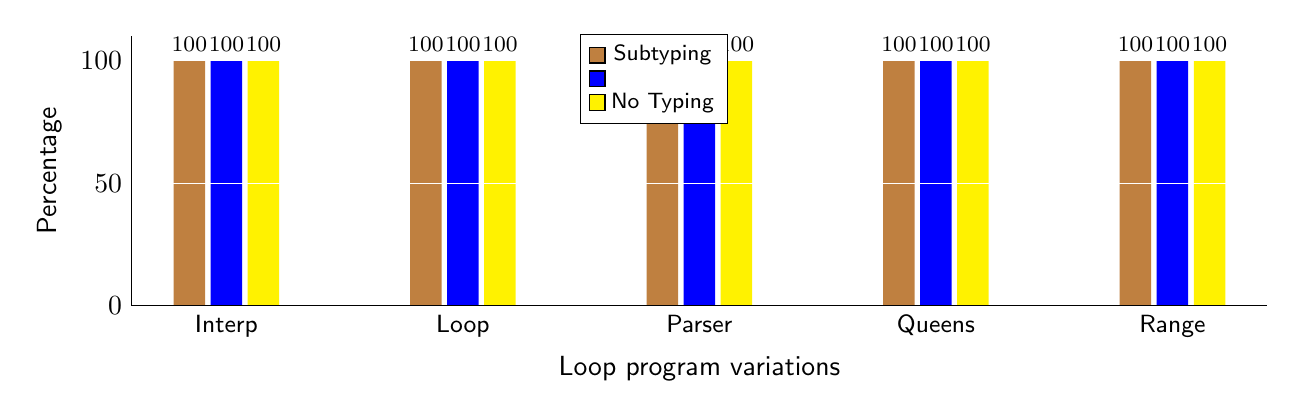
\begin{tikzpicture}
    \centering
    \begin{axis}[
        ybar, axis on top,
        height=5cm, width=16cm,
        ymajorgrids, tick align=inside,
        bar width=0.4cm,
        major grid style={draw=white},
        enlarge y limits={value=.1,upper},
        ymin=0, ymax=100,
        axis x line*=bottom,
        axis y line*=left,
        y axis line style={opacity=1},
        tickwidth=0pt,
        xtick = data,
        x tick label style={font=\small,text width=1.4cm,align=center},
            enlarge x limits=true,
        legend image code/.code={%
        \draw[#1] (0cm,-0.1cm) rectangle (0.2cm,0.1cm);
    },
            legend style={
            at={(0.46,1.01)},
            anchor=north,
            % legend columns=-1,
            % /tikz/every even column/.append style={column sep=0.4cm},
            font = \footnotesize
        },
        ylabel={Percentage},
        xlabel={Loop program variations},
            symbolic x coords={
            Interp,
            Loop,
            Parser,
            Queens,
            Range,
            },
            nodes near coords={
            \footnotesize \pgfmathprintnumber{\pgfplotspointmeta}
        }
    ]
    \addplot [draw=none,fill=brown] coordinates {
        (Interp,100)
        (Loop,100)
        (Parser,100)
        (Queens,100)
        (Range,100)
    };

    \addplot [draw=none,fill=blue] coordinates {
        (Interp,100)
        (Loop,100)
        (Parser,100)
        (Queens,100)
        (Range,100)
    };

    \addplot [draw=none,fill=yellow] coordinates {
        (Interp,100)
        (Loop,100)
        (Parser,100)
        (Queens,100)
        (Range,100)
    };
    
    \legend{Subtyping, \core, No Typing}
    \end{axis}
    \end{tikzpicture}
\caption{Relative run-times of testing programs}
\label{fig:test}
\end{figure}
    
\subsection{Type Inference Comparison}

The main contribution of this thesis is to extend the algebraic subtyping algorithm with algebraic effects and handlers. The goal is to be able to infer types which are shorter, simpler and more human-readable than types inferred by standard subtyping systems. In this evaluation, several small programs were made and its types inferred by the subtyping and the algebraic subtyping system in order to compare both types. 

Considering that the implementation does not yet support the simplification of types, the results are inaccurate. In order to provide a proper evaluation, the types have been manually simplified using the simplification algorithm. All three types are given in order to the current state of the implementation and to be able to evaluate the algebraic subtyping system.


\todo{give the evaluation results}

\begin{figure}[H]
\begin{center}
\begin{framed}
\begin{minipage}[t]{0.95\columnwidth}
    \begin{mathpar}
    \inferrule[Interp]{}{
        \ctxp \prinent x \T [x : \alpha]\alpha
    }

    \inferrule[Loop]{}{
        \ctxp \prinent x \T [x : \alpha]\alpha
    }

    \inferrule[Parser]{}{
        \ctxp \prinent x \T [x : \alpha]\alpha
    }

    \inferrule[Queens]{}{
        \ctxp \prinent x \T [x : \alpha]\alpha
    }

    \inferrule[Range]{}{
        \ctxp \prinent x \T [x : \alpha]\alpha
    }
\end{mathpar}
\end{minipage}
\end{framed}
\end{center}
\caption{Produced types for Subtyping}\label{fig:inferred:sub}
\end{figure}

\begin{figure}[H]
\begin{center}
\begin{framed}
\begin{minipage}[t]{0.95\columnwidth}
    \begin{mathpar}
    \inferrule[Interp]{}{
        \ctxp \prinent x \T [x : \alpha]\alpha
    }

    \inferrule[Loop]{}{
        \ctxp \prinent x \T [x : \alpha]\alpha
    }

    \inferrule[Parser]{}{
        \ctxp \prinent x \T [x : \alpha]\alpha
    }

    \inferrule[Queens]{}{
        \ctxp \prinent x \T [x : \alpha]\alpha
    }

    \inferrule[Range]{}{
        \ctxp \prinent x \T [x : \alpha]\alpha
    }
\end{mathpar}
\end{minipage}
\end{framed}
\end{center}
\caption{Produced types for \core}\label{fig:inferred:core}
\end{figure}

\begin{figure}[H]
\begin{center}
\begin{framed}
\begin{minipage}[t]{0.95\columnwidth}
    \begin{mathpar}
    \inferrule[Interp]{}{
        \ctxp \prinent x \T [x : \alpha]\alpha
    }

    \inferrule[Loop]{}{
        \ctxp \prinent x \T [x : \alpha]\alpha
    }

    \inferrule[Parser]{}{
        \ctxp \prinent x \T [x : \alpha]\alpha
    }

    \inferrule[Queens]{}{
        \ctxp \prinent x \T [x : \alpha]\alpha
    }

    \inferrule[Range]{}{
        \ctxp \prinent x \T [x : \alpha]\alpha
    }
\end{mathpar}
\end{minipage}
\end{framed}
\end{center}
\caption{Produced types for Algebraic Subtyping}\label{fig:inferred:manual}
\end{figure}

\section{Conclusion}

\section{Future Work}
\todo{write future work}

\subsection{Simplification}

\subsection{Biunification with type automata}

\subsection{Optimization}

\section{Conclusion}

\todo{write conclusion}
Briefly recall what the goal of the work was. Summarize what you have done, summarize the results, and present conclusions. Conclusions include a critical assessment: where the original goals reached? Discuss the limitations of your work. Describe how the work could possibly be extended in the future, mitigating limitations or solving remaining problems.



\appendixpage*          % if wanted
\appendix
% \chapter{Appendix A}
% \input{tex/appendix}

\backmatter

% The bibliography comes after the appendices.
% You can replace the standard "abbrv" bibliography style by another one.
\bibliographystyle{abbrv}
\bibliography{bib/main}

\end{document}
